% ==================================================================
% ERW — Ex-Ante Modelling in Sub-Saharan Africa: End-to-End Technical Report
% Bisrat's house-style report (bisrat-latex-report skill):
% book class · APA citations (apacite + natbib) · blue hyperlinks.
%
% Hand-authored. Build with:
%   docs/build-erw-technical-report.sh
% Manually: xelatex -> bibtex -> xelatex -> xelatex
% xelatex is required for inline Unicode (micro sign, degree, arrows).
% ==================================================================

\PassOptionsToPackage{hyphens}{url}
\documentclass[openany]{book}
\usepackage{amsmath,amssymb}
\usepackage{lmodern}
\usepackage[sectionbib]{chapterbib}
\usepackage[%
% numberedbib,
natbibapa
]{apacite}

\usepackage{hyperref}
\usepackage[figuresright]{rotating}

\usepackage{xcolor}
\definecolor{callout}{HTML}{F2F6FA}
\definecolor{calloutrule}{HTML}{2c5f8a}
\hypersetup{
    colorlinks=true,
    linkcolor=blue,
    linkbordercolor=blue,
    citecolor=blue,
    filecolor=cyan,
    urlcolor=blue,
    pdftitle={ERW: Ex-Ante Modelling in Sub-Saharan Africa --- End-to-End Technical Report},
    pdfauthor={Bisrat Haile},
    pdfcreator={LaTeX}
}
\usepackage{iftex}
\usepackage{multirow}
\ifPDFTeX
  \usepackage[T1]{fontenc}
  \usepackage[utf8]{inputenc}
  \usepackage{textcomp}
\else
  \usepackage{unicode-math}
  \defaultfontfeatures{Scale=MatchLowercase}
  \defaultfontfeatures[\rmfamily]{Ligatures=TeX,Scale=1}
  \setmainfont{Helvetica Neue}
  \setmonofont{Menlo}
\fi
\IfFileExists{upquote.sty}{\usepackage{upquote}}{}
\IfFileExists{microtype.sty}{%
  \usepackage[]{microtype}
  \UseMicrotypeSet[protrusion]{basicmath}
}{}
\makeatletter
\@ifundefined{KOMAClassName}{%
  \IfFileExists{parskip.sty}{%
    \usepackage{parskip}
  }{%
    \setlength{\parindent}{0pt}
    \setlength{\parskip}{6pt plus 2pt minus 1pt}}
}{%
  \KOMAoptions{parskip=half}}
\makeatother

\usepackage{longtable,booktabs,array}
\newcounter{none}
\usepackage{calc}
\usepackage{etoolbox}
\makeatletter
\patchcmd\longtable{\par}{\if@noskipsec\mbox{}\fi\par}{}{}
\makeatother
\IfFileExists{footnotehyper.sty}{\usepackage{footnotehyper}}{\usepackage{footnote}}
\makesavenoteenv{longtable}
\usepackage{graphicx}
\usepackage{float}
\usepackage{subcaption}
\usepackage{mdframed}
\makeatletter
\def\maxwidth{\ifdim\Gin@nat@width>\linewidth\linewidth\else\Gin@nat@width\fi}
\def\maxheight{\ifdim\Gin@nat@height>\textheight\textheight\else\Gin@nat@height\fi}
\makeatother
\setkeys{Gin}{width=\maxwidth,height=\maxheight,keepaspectratio}
\makeatletter
\def\fps@figure{H}
\makeatother
\setlength{\emergencystretch}{3em}
\providecommand{\tightlist}{%
  \setlength{\itemsep}{0pt}\setlength{\parskip}{0pt}}
\setcounter{secnumdepth}{4}
\ifLuaTeX
  \usepackage{selnolig}
\fi

% Compact chapter headings: "3. Title" inline, not "Chapter 3" on its own line.
\usepackage{titlesec}
\titleformat{\chapter}[hang]{\Huge\bfseries}{\thechapter.}{12pt}{}
\titleformat{name=\chapter,numberless}[hang]{\Huge\bfseries}{}{0pt}{}
\titlespacing*{\chapter}{0pt}{6pt}{24pt}

\setlength{\tabcolsep}{4pt}
\renewcommand{\arraystretch}{1.08}

% A light callout box for key-idea asides.
\newmdenv[
  backgroundcolor=callout,
  linecolor=calloutrule,
  linewidth=1.2pt,
  topline=false,rightline=false,bottomline=false,
  leftline=true,
  innertopmargin=8pt,innerbottommargin=8pt,
  innerleftmargin=10pt,innerrightmargin=10pt,
  skipabove=8pt,skipbelow=8pt
]{keybox}

% Shorthand
\newcommand{\co}{\ensuremath{\mathrm{CO_2}}}
\newcommand{\tco}{\ensuremath{\mathrm{tCO_2}}}
\newcommand{\um}{\ensuremath{\mu\mathrm{m}}}

% ---- Title block ------------------------------------------------
\title{\huge{\textbf{ERW:}} \textsc{Ex-Ante Modelling in Sub-Saharan Africa}}
\makeatletter
\providecommand{\subtitle}[1]{%
  \apptocmd{\@title}{\par {\large #1 \par}}{}{}
}
\makeatother
\subtitle{\textsc{\large \textbf{An end-to-end technical report on the modelling
approach: workflow, equations, assumptions, and results}}}
\author{\href{mailto:bismignot@gmail.com}{Bisrat Haile}\\CIMMYT}
\date{Last updated: \today}

\begin{document}
\frontmatter
\maketitle
\tableofcontents
\newpage
\listoffigures
\listoftables
\mainmatter

% ==================================================================
\chapter*{About this report}
\addcontentsline{toc}{chapter}{About this report}
\markboth{ABOUT THIS REPORT}{ABOUT THIS REPORT}

This report documents, end to end, the ex-ante model that maps where Enhanced
Rock Weathering (ERW) with crushed basalt is likely to be worthwhile on
Sub-Saharan African (SSA) cropland. It explains the \emph{workflow} (which
script computes what, in what order), the \emph{equations} (every mechanism and
constant, drawn directly from the code), the \emph{modelling choices} (why the
model is shaped the way it is, and where it uses defensible proxies), and the
\emph{results} produced under the current defaults.

\textbf{What this model is.} It is a spatially explicit \emph{screening} model.
It ranks and compares locations, quantifies the two returns ERW can generate ---
durable carbon dioxide removal (a public good) and an agronomic liming
co-benefit (a private good) --- and stress-tests those returns against price,
yield, and logistics assumptions. It is deliberately transparent and fast: every
term is an interpretable multiplier that can be traced to a published anchor.

\textbf{What this model is not.} It is not a monitoring, reporting and
verification (MRV) or carbon-crediting instrument. The absolute per-hectare
tonnages it reports are order-of-magnitude estimates, not bankable credits;
credit-grade numbers require mechanistic reactive-transport modelling and field
measurement (\autoref{ch:roadmap}). Read the tonnages as a way to compare
pixels, not to certify them.

\textbf{Relationship to the other documents.} Two companion documents go deeper
on specific pieces: the \emph{Carbon Dioxide Removal --- Technical Derivation}
(\texttt{erw-cdr-calculations.pdf}) sources every step of the CDR stoichiometry
and net-export accounting; the \emph{parameters and assumptions} catalogue
(\texttt{erw-parameters.md}) is the master list of constants with citations.
This report is the integrating narrative that ties the whole pipeline together.

Headline numbers are quoted from the model run dated 2026-05-26 unless stated
otherwise. Where a worked example uses earlier defaults, this is flagged; the
equations are unchanged, only the input constants differ.

% ==================================================================
\chapter{Introduction and scope}\label{ch:intro}

\section{What Enhanced Rock Weathering does}

Silicate rocks weather naturally: rain-derived carbonic acid attacks the
minerals, the acid is consumed, and the carbon leaves as dissolved bicarbonate.
Over geological time this is one of Earth's principal thermostats. Enhanced Rock
Weathering simply accelerates it --- grind a fast-weathering silicate such as
basalt to a powder, spread it on a field, and the vastly increased mineral
surface area lets the reaction run in years rather than millennia
\citep{hartmann2013, beerling2020}. For a divalent cation such as calcium, the
net reaction consumes two moles of \co\ per mole of cation released:
%
\begin{equation}
\mathrm{CaSiO_3} + 2\,\mathrm{CO_2} + 3\,\mathrm{H_2O}
\;\longrightarrow\;
\mathrm{Ca^{2+}} + 2\,\mathrm{HCO_3^-} + \mathrm{H_4SiO_4}.
\label{eq:weathering}
\end{equation}
%
The captured carbon is durable for $10^3$--$10^5$ years once it reaches the
ocean as bicarbonate \citep{renforth2019, kanzaki2023}.

ERW is attractive on \emph{cropland} for a second reason. The alkalinity that
basalt releases is chemically the same medicine that agricultural lime
delivers: it raises pH and neutralises the exchangeable acidity and aluminium
toxicity that suppress yields on the acidic soils common across the tropics.
So a single application can pay twice --- a durable carbon credit (the
\emph{public} return) and a yield uplift the farmer keeps (the \emph{private}
return). Much of SSA has the acidic, weathered soils, the warm-wet climate that
speeds weathering, and the smallholder yield gap that makes this pairing
compelling \citep{beerling2020, baek2023}.

\section{The question the model answers}

Given all of the above, \emph{where} on SSA cropland is ERW worth doing, for whom,
and how sensitive is that answer to what we assume? The model answers this pixel
by pixel and crop by crop, holding the biogeochemistry, agronomy, and
economic geography in one accounting identity (\autoref{ch:framework}).

\section{Scope and units}

\begin{keybox}
\textbf{At a glance.} $\sim$9\,km working grid (SoilGrids-Africa aggregated
$10\times$), 47 SSA countries, 23 SPAM crops, all monetary values in USD, a
5-year project horizon, and a per-pixel / farmer's-eye accounting perspective.
\end{keybox}

\begin{longtable}[]{@{}ll@{}}
\caption{Spatial, temporal, and accounting scope of the model.}\label{tbl:scope}\\
\toprule
Dimension & Setting \\
\midrule
\endfirsthead
\toprule
Dimension & Setting \\
\midrule
\endhead
Region & Sub-Saharan Africa, 47 countries (GADM v4); islands excluded \\
Working grid & SoilGrids-Africa $30''$ aggregated $10\times \approx 0.083^\circ$ ($\sim$9\,km) \\
Land mask & QED cropland, pixels with $>10\%$ cropland fraction \\
Crops & 23 SPAM v2 crops (cereals, legumes, commodities, roots \& tubers) \\
Horizon & 5 years (industry accreditation window) \\
Currency & USD throughout \\
Perspective & Per pixel, farmer's-eye; no aggregator-level finance \\
Feedstock & Basalt (mafic silicate); ultramafics excluded (Ni/Cr risk) \\
\bottomrule
\end{longtable}

The remainder of the report follows the model's own logic: the scientific
framework (\autoref{ch:framework}), the pipeline and data
(\autoref{ch:pipeline}), then each computational block --- feedstock and rate
(\autoref{ch:feedstock}), CDR (\autoref{ch:cdr}), crop response
(\autoref{ch:crop}), cost and logistics (\autoref{ch:cost}), profitability
(\autoref{ch:profit}), and supply and sensitivity (\autoref{ch:supply}) --- and
closes with results (\autoref{ch:results}), limitations and roadmap
(\autoref{ch:roadmap}), and reproducibility (\autoref{ch:repro}).

% ==================================================================
\chapter{Scientific framework}\label{ch:framework}

The model decomposes the value of a basalt application into three independent
``streams'' that are computed separately and then reconciled in a single
per-pixel gross-margin identity (\autoref{fig:framework}).

\begin{figure}
  \centering
  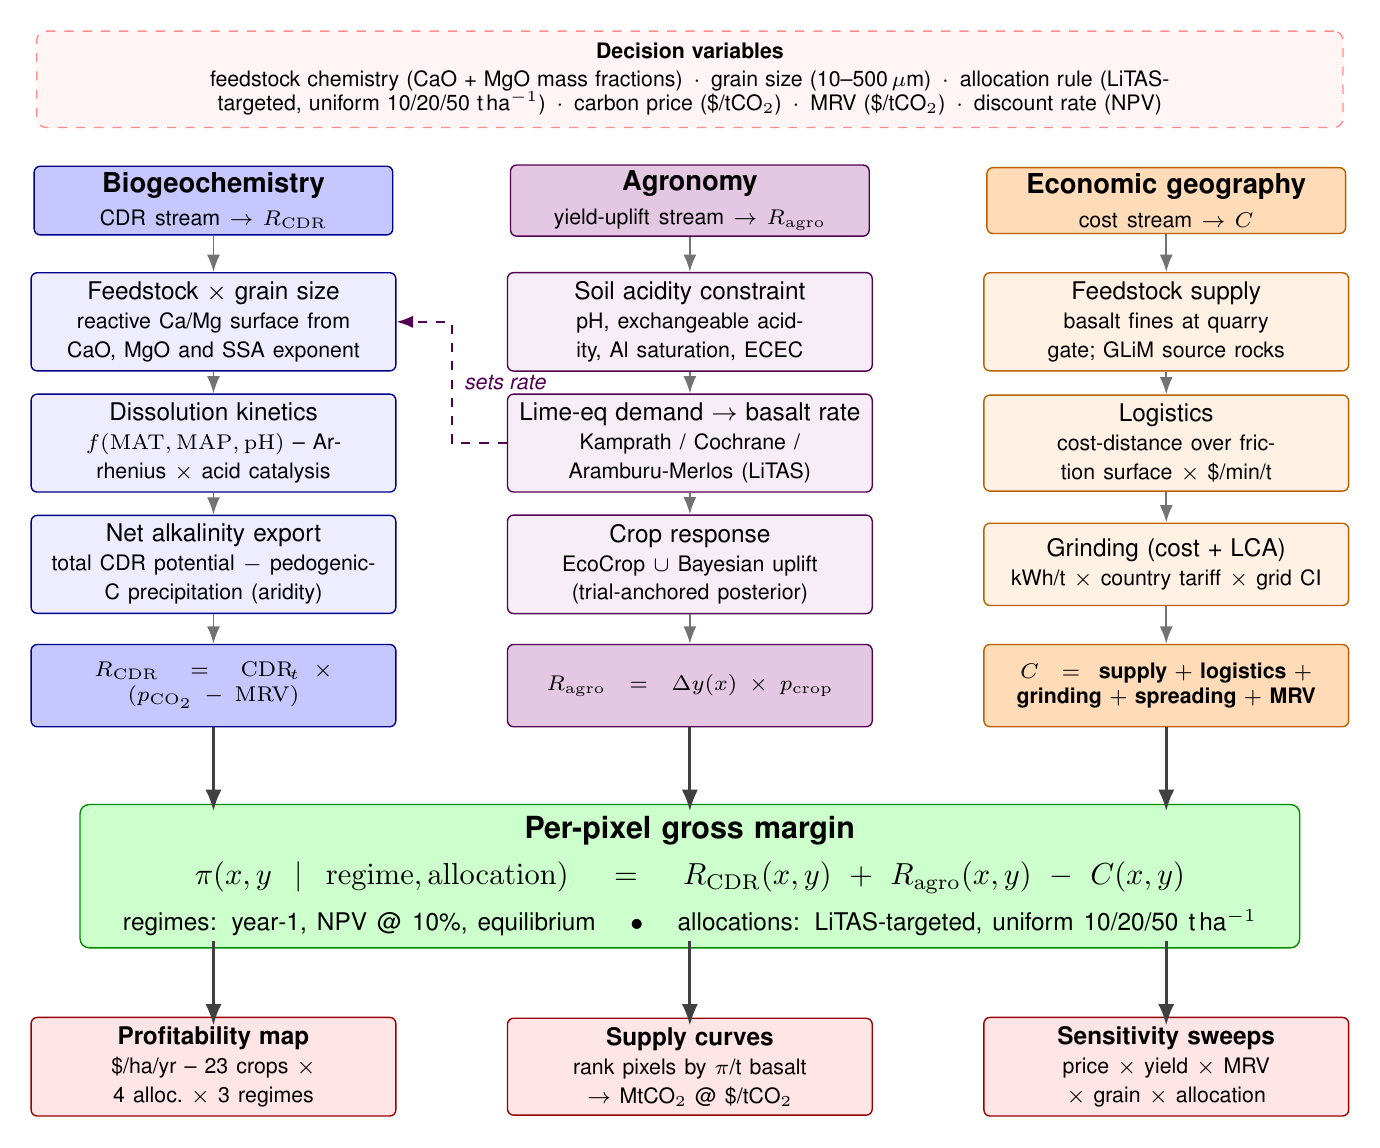
\includegraphics[width=\linewidth]{erw-conceptual-framework.png}
  \caption{The three-stream conceptual framework. A biogeochemical stream turns
  basalt into durable CDR ($R_{\mathrm{CDR}}$); an agronomic stream turns the
  same alkalinity into a yield uplift ($R_{\mathrm{agro}}$); an
  economic-geography stream builds up the delivered-and-applied cost ($C$).
  The dashed cross-arrow marks the coupling: the agronomic lime demand
  \emph{sets the application rate} that both other streams then scale.}
  \label{fig:framework}
\end{figure}

\section{The three streams}

\begin{description}
\item[Biogeochemistry $\rightarrow R_{\mathrm{CDR}}$.] From feedstock chemistry
and grain size, through dissolution kinetics that respond to temperature,
moisture and pH, to the net alkalinity actually exported (total capture minus
the fraction that re-precipitates locally as pedogenic carbonate). Detailed in
\autoref{ch:feedstock} and \autoref{ch:cdr}.
\item[Agronomy $\rightarrow R_{\mathrm{agro}}$.] From the soil acidity
constraint (pH, exchangeable acidity, aluminium saturation, ECEC) to a
lime-equivalent demand, which both sets the basalt rate and --- via a crop
suitability response --- implies a yield uplift. Detailed in \autoref{ch:crop}.
\item[Economic geography $\rightarrow C$.] From feedstock supply at the quarry
gate, through cost-distance logistics over a friction surface, grinding energy
priced at the local electricity tariff, spreading, and MRV. Detailed in
\autoref{ch:cost}.
\end{description}

\section{The master identity}

For a pixel at location $x$ growing crop $y$, under a chosen accounting regime
and allocation rule, the per-pixel gross margin is
%
\begin{equation}
\pi(x,y \mid \text{regime},\text{allocation})
= R_{\mathrm{CDR}}(x,y) + R_{\mathrm{agro}}(x,y) - C(x,y).
\label{eq:master}
\end{equation}
%
Everything downstream --- profitability maps, supply curves, sensitivity sweeps
--- is a transformation of \autoref{eq:master}. The \emph{decision variables}
(the dials a project designer can turn) are feedstock chemistry, grain size,
allocation rule (targeted lime-requirement dose vs.\ uniform 10/20/50\,t\,ha$^{-1}$),
carbon price, MRV cost, and discount rate.

\begin{keybox}
\textbf{Why the streams are coupled, not independent.} The agronomic
lime-requirement calculation produces the \emph{rate} (t\,ha$^{-1}$) of basalt.
That single rate then multiplies both the CDR per hectare and the cost per
hectare. Applying more basalt buys more carbon and more yield relief, but also
more cost and more lifecycle emissions --- which is why the ``right'' rate is a
genuine optimisation, not a maximisation (\autoref{ch:supply}).
\end{keybox}

% ==================================================================
\chapter{Pipeline architecture and data}\label{ch:pipeline}

\section{Nine blocks, one dependency graph}

The pipeline is implemented as a chain of R scripts (prefix \texttt{erw-})
organised into nine functional blocks, B1--B9 (\autoref{fig:pipeline}). Each
script reads rasters written by its predecessors and writes rasters for its
successors; there is no hidden state.

\begin{figure}
  \centering
  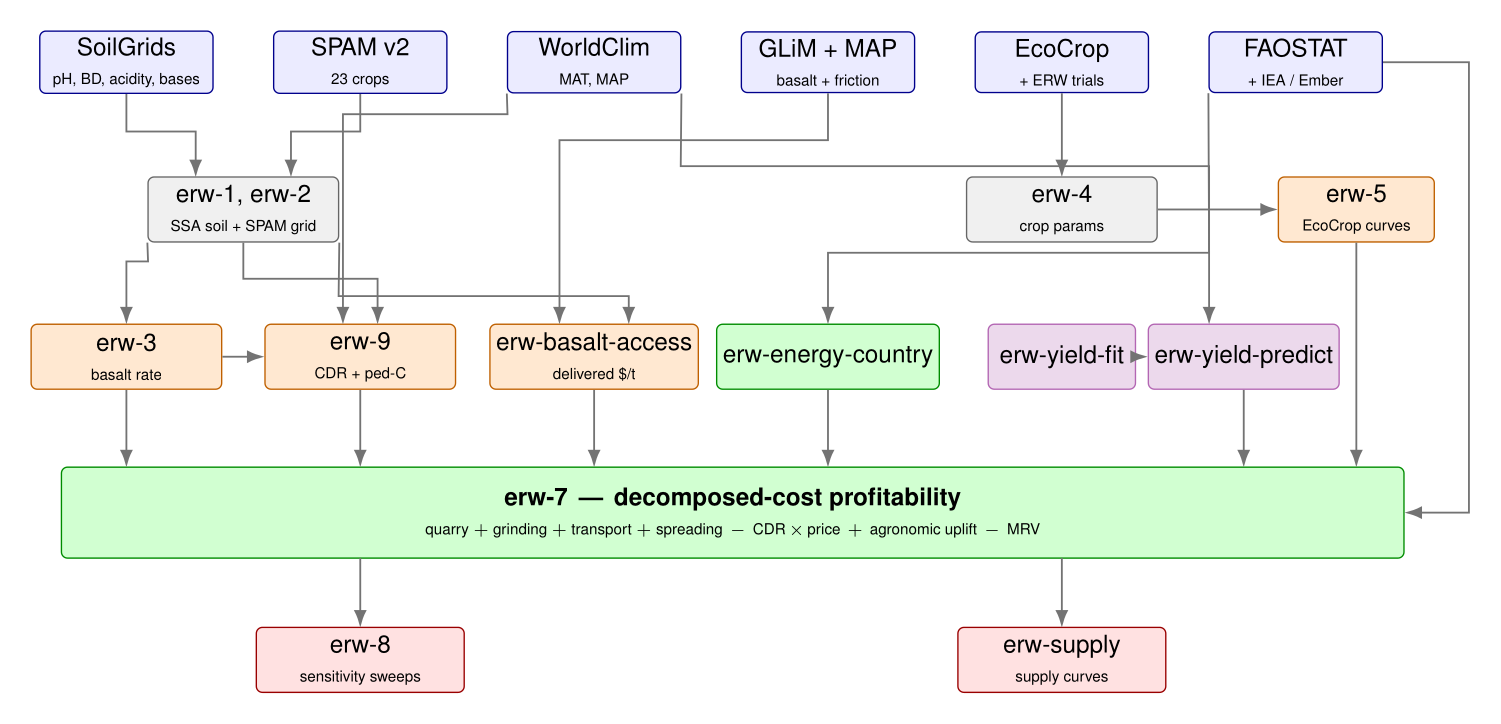
\includegraphics[width=\linewidth]{erw-pipeline-flow.png}
  \caption{Pipeline architecture. Blue = raw data sources; grey = the common
  working grid; orange = geospatial surfaces; green = energy; purple = the
  (optional) Bayesian yield arm; the wide green bar = the profitability engine
  (\texttt{erw-7}); red = deliverables. Arrows are data dependencies.}
  \label{fig:pipeline}
\end{figure}

\begin{longtable}[]{@{}l>{\raggedright\arraybackslash}p{3.7cm}>{\raggedright\arraybackslash}p{6.3cm}@{}}
\caption{The nine blocks and the scripts that implement them.}\label{tbl:blocks}\\
\toprule
Block & Script(s) & What it produces \\
\midrule
\endfirsthead
\toprule
Block & Script(s) & What it produces \\
\midrule
\endhead
B1 Grid & \texttt{erw-1}, \texttt{erw-2} & SSA + cropland mask; depth-weighted
soil stack; SPAM area/production/yield for 23 crops \\
B2 Rate & \texttt{erw-3} & Lime-equivalent demand $\rightarrow$ basalt rate;
feedstock chemistry; uniform-rate rasters \\
B6 Crop & \texttt{erw-4}, \texttt{erw-5} & Per-crop EcoCrop pH and acidity
tolerance tables and relative-yield rasters \\
B3 CDR & \texttt{erw-9} & Climate/pH-scaled, pedogenic-deducted, net-export
CDR per hectare \\
B4 Logistics & \texttt{erw-basalt-access} (+ \texttt{build-basalt-mask},
\texttt{fetch-friction-surface}) & Basalt sources; travel time; delivered
price \\
B5 Energy & \texttt{erw-energy-country} & Country electricity tariff and grid
carbon intensity \\
(B6$'$) Bayesian & \texttt{erw-yield-fit}, \texttt{erw-yield-predict} &
Trial-anchored per-crop uplift rasters (optional; not run at v1) \\
B7 Profit & \texttt{erw-7} & Decomposed-cost gross margin: 4 allocations
$\times$ 3 regimes $\times$ 23 crops = 276 rasters \\
B8 Supply & \texttt{erw-supply} & Pixel ranking by GM per tonne basalt; supply
curves \\
B9 Sensitivity & \texttt{erw-8} & Five parameter sweeps \\
\bottomrule
\end{longtable}

\section{Data sources}

\begin{longtable}[]{@{}lp{5.4cm}l@{}}
\caption{External datasets and their roles.}\label{tbl:data}\\
\toprule
Dataset & Provides & Source \\
\midrule
\endfirsthead
\toprule
Dataset & Provides & Source \\
\midrule
\endhead
SoilGrids-Africa & pH, bulk density, exch.\ acidity, exch.\ bases (K/Ca/Mg/Na) &
\citet{poggio2021} \\
SPAM v2 & Harvested area, production, yield, 23 crops & \citet{yu2020} \\
WorldClim 2.1 & Mean annual temperature, precipitation & \citet{fick2017} \\
GLiM v1 & Basalt-source lithology (basic volcanic, pyroclastic, gabbro) &
\citet{hartmann2012} \\
MAP friction surface & Motorised travel-time friction & \citet{weiss2020} \\
EcoCrop / Recocrop & Crop pH and acidity tolerance envelopes & \citet{recocrop} \\
FAOSTAT & Producer prices (2016--2020 SSA median) & \citet{faostat} \\
Ember / IEA & Grid carbon intensity, electricity tariffs & country table \\
CGIAR-CSI & Global Aridity Index (pedogenic deduction) & \citet{zomer2022} \\
\bottomrule
\end{longtable}

\section{Building the working grid (B1)}

\texttt{erw-1} defines SSA (GADM v4, dropping island states), applies the QED
cropland filter (keep pixels $>10\%$ cropland), and assembles the SoilGrids
soil-property stack. Soil properties are \emph{depth-weighted} over the top
30\,cm,
%
\begin{equation}
p \;=\; \frac{5\,p_{5} + 10\,p_{15} + 15\,p_{30}}{30},
\label{eq:depthweight}
\end{equation}
%
and two derived layers are formed inline: the effective cation exchange capacity
$\mathrm{ECEC} = \mathrm{H^{+}_{exch}} + \sum(\mathrm{K,Ca,Mg,Na})$ and the
acidity saturation $\mathrm{H^{+}_{sat}} = 100\,\mathrm{H^{+}_{exch}}/\mathrm{ECEC}$
(\%). \texttt{erw-2} pulls SPAM v2 for all 23 crops and resamples everything onto
the common $10\times$-aggregated grid, so every later raster is co-registered.

% ==================================================================
\chapter{Feedstock chemistry and the basalt rate}\label{ch:feedstock}

This block (\texttt{erw-3}) answers two coupled questions: \emph{how much} basalt
to apply (the rate), and \emph{how much carbon} a tonne of it could remove (the
per-tonne ceiling, before spatial de-rating in \autoref{ch:cdr}).

\section{Feedstock composition}

Basalt is represented by a small set of oxide mass fractions
(\autoref{tbl:chem}); only CaO and MgO are consumed in the current CDR
stoichiometry (K, Na, P are carried for future nutrient accounting; Ni and Cr
are carried as a contamination-risk surrogate).

\begin{longtable}[]{@{}lll@{}}
\caption{Default basalt chemistry (mass fractions unless noted).}\label{tbl:chem}\\
\toprule
Component & Default & Role \\
\midrule
\endhead
CaO & 0.10 & Cation source (consumed) \\
MgO & 0.07 & Cation source (consumed) \\
K$_2$O & 0.015 & Nutrient (not yet consumed) \\
Na$_2$O & 0.025 & Carried, not consumed \\
P$_2$O$_5$ & 0.003 & Nutrient (not yet consumed) \\
Ni & 100\,ppm & Contamination-risk surrogate \\
Cr & 200\,ppm & Contamination-risk surrogate \\
Grain size $d$ & 50\,\um & Decision variable \\
Reactive fraction $\phi_0$ & 0.20 & Fraction of stoichiometric limit realised \\
\bottomrule
\end{longtable}

\section{Stoichiometric ceiling}

Using standard oxide-to-product mass ratios (1\,g CaO $\rightarrow$ 1.783\,g
CaCO$_3$-eq and 1.570\,g \co; 1\,g MgO $\rightarrow$ 2.481\,g CaCO$_3$-eq and
2.185\,g \co), the calcium-carbonate equivalent and the stoichiometric CDR
ceiling per tonne of basalt are
%
\begin{align}
\mathrm{CCE} &= 0.10\times 1.783 + 0.07\times 2.481 \approx 0.352
  \;\;(\text{352\,kg CaCO}_3/\text{t}), \label{eq:cce}\\
\mathrm{CDR_{max}} &= \big(0.10\times 1.570 + 0.07\times 2.185\big)\times 1000
  \approx \mathbf{310}\ \text{kg \co/t basalt}. \label{eq:cdrmax}
\end{align}
%
\autoref{eq:cdrmax} is a hard upper bound --- the carbon captured if every
calcium and magnesium ion weathered and every bicarbonate reached the ocean.
Reality is a fraction of it, and quantifying that fraction is the whole task of
\autoref{ch:cdr}.

\section{Grain size: a reactivity--energy trade-off}

Grinding finer exposes more surface area (more reactivity) but costs more energy
(more cost and lifecycle emissions). Both sides are power laws anchored to the
literature. The reactivity (surface-area) factor, relative to a 100\,\um\
reference, uses exponent $\beta=0.5$:
%
\begin{equation}
f_{\text{grain}} = \left(\frac{100}{d}\right)^{0.5},
\qquad f_{\text{grain}}(50\,\um) = \sqrt{2}\approx 1.414.
\label{eq:grain}
\end{equation}
%
Grinding energy follows the Strefler curve (0.07\,GJ/t at 50\,\um, exponent
$\alpha=1.2$; \citealp{strefler2018}):
%
\begin{equation}
E_{\text{grind}}(d) = 0.07\left(\frac{50}{d}\right)^{1.2}\ \text{GJ/t},
\qquad \text{kWh/t} = E_{\text{grind}}\times 277.78.
\label{eq:grind}
\end{equation}
%
At the 50\,\um\ default this is 19.4\,kWh/t. Grain size is a decision variable
precisely because \autoref{eq:grain} and \autoref{eq:grind} pull in opposite
directions; \autoref{ch:supply} sweeps it.

\section{From lime demand to basalt rate}

The \emph{effective neutralising value} folds the reactive fraction and grain
factor into the CCE, and its reciprocal converts a lime requirement into a
basalt rate:
%
\begin{equation}
\mathrm{NV_{eff}} = \mathrm{CCE}\cdot\phi_0\cdot f_{\text{grain}},
\qquad r_{\text{bl}} = \frac{1}{\mathrm{NV_{eff}}}.
\label{eq:nv}
\end{equation}
%
At the 50\,\um\ default, $\mathrm{NV_{eff}}\approx 0.10$ so
$r_{\text{bl}}\approx 10.0$ t basalt per t CaCO$_3$-equivalent. The reference
per-tonne CDR that \autoref{ch:cdr} scales spatially is
$\mathrm{CDR_{eff}} = \mathrm{CDR_{max}}\cdot\phi_0\cdot f_{\text{grain}}
\approx 88$\,kg \co/t.

The lime requirement $L$ itself comes from the \texttt{limer} engine, which
implements three published tropical-soil methods --- Kamprath, Cochrane, and the
Aramburu-Merlos LiTAS (``lime to a target acidity saturation'') model
\citep{aramburu2023}. The targeted basalt rate is
%
\begin{equation}
R_{\text{targeted}} = L \times r_{\text{bl}} \quad (\text{t basalt ha}^{-1}),
\label{eq:rate}
\end{equation}
%
applied only where acidity saturation exceeds a threshold ($>10\%$, and, per
crop, above the crop's own tolerance; \autoref{ch:crop}). The counterfactual
\emph{uniform} rules apply a flat 10, 20, or 50\,t\,ha$^{-1}$ everywhere there is
cropland, matching the convention of continental studies
\citep{beerling2020, baek2023}. \autoref{fig:rate-map} shows the resulting
LiTAS rate.

\begin{figure}
  \centering
  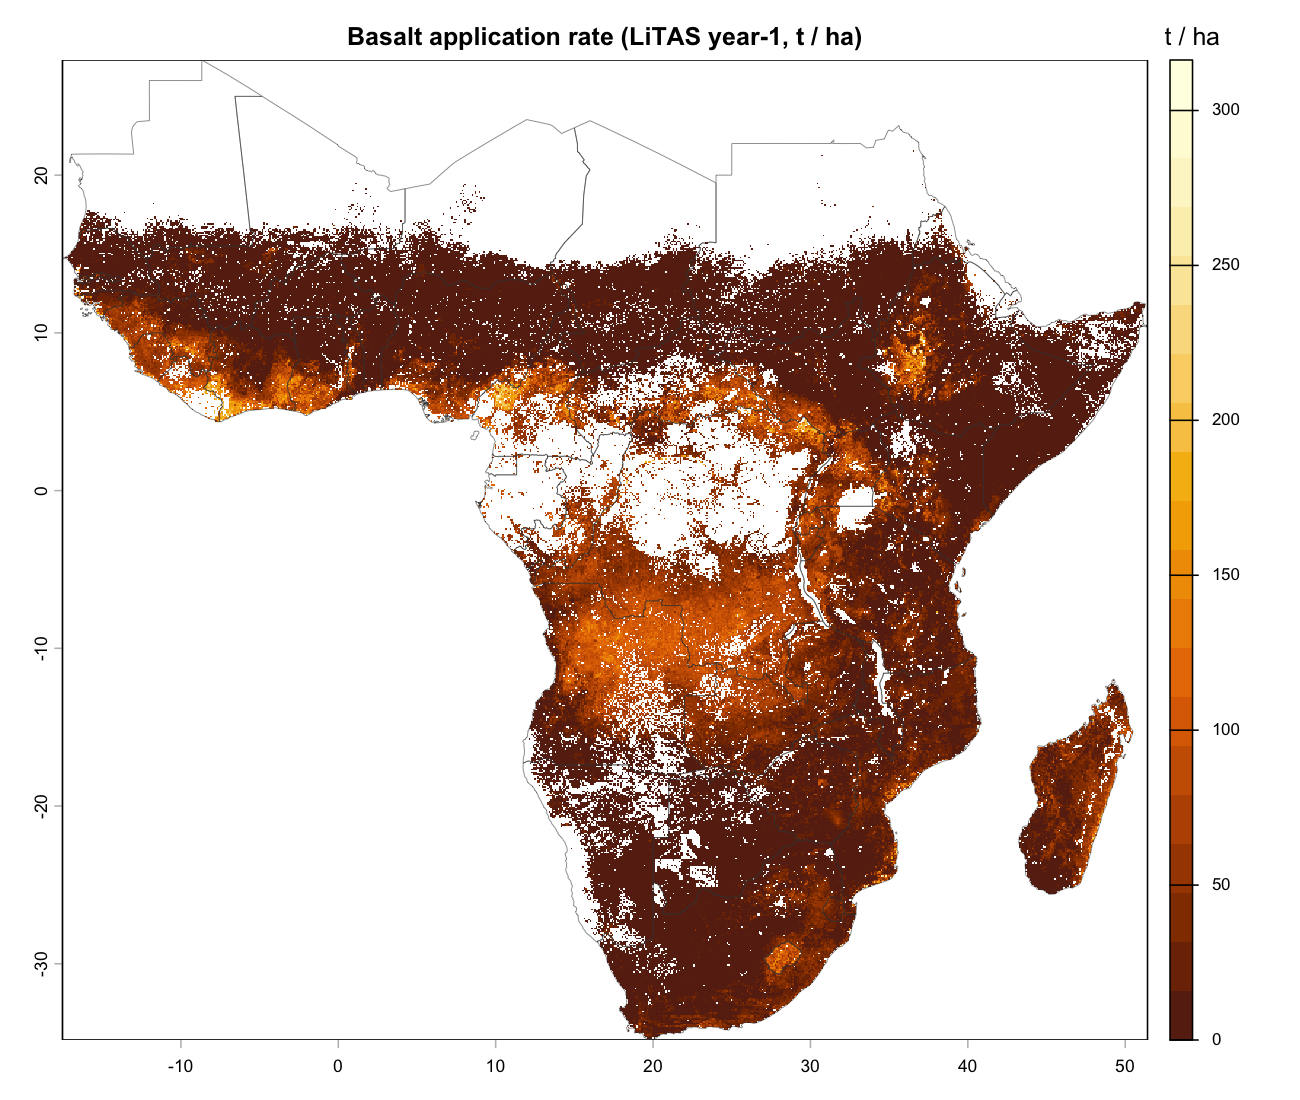
\includegraphics[width=0.82\linewidth]{maps/02-basalt-rate-merlos.png}
  \caption{Targeted (LiTAS) basalt application rate, t\,ha$^{-1}$. High where
  soils are strongly acidic and lime demand is large; zero on near-neutral
  soils, which the targeted rule skips.}
  \label{fig:rate-map}
\end{figure}

% ==================================================================
\chapter{The carbon-dioxide-removal surface}\label{ch:cdr}

The stoichiometric ceiling of \autoref{eq:cdrmax} is de-rated, pixel by pixel,
by three physical realities: not all of the mineral reacts (reactive fraction,
scaled by climate), some of the released alkalinity re-precipitates locally as
carbonate (pedogenic loss), and some is spent neutralising the soil's own
acidity rather than being exported (net-export correction). The cascade is
summarised in \autoref{fig:cascade}.

\begin{figure}
  \centering
  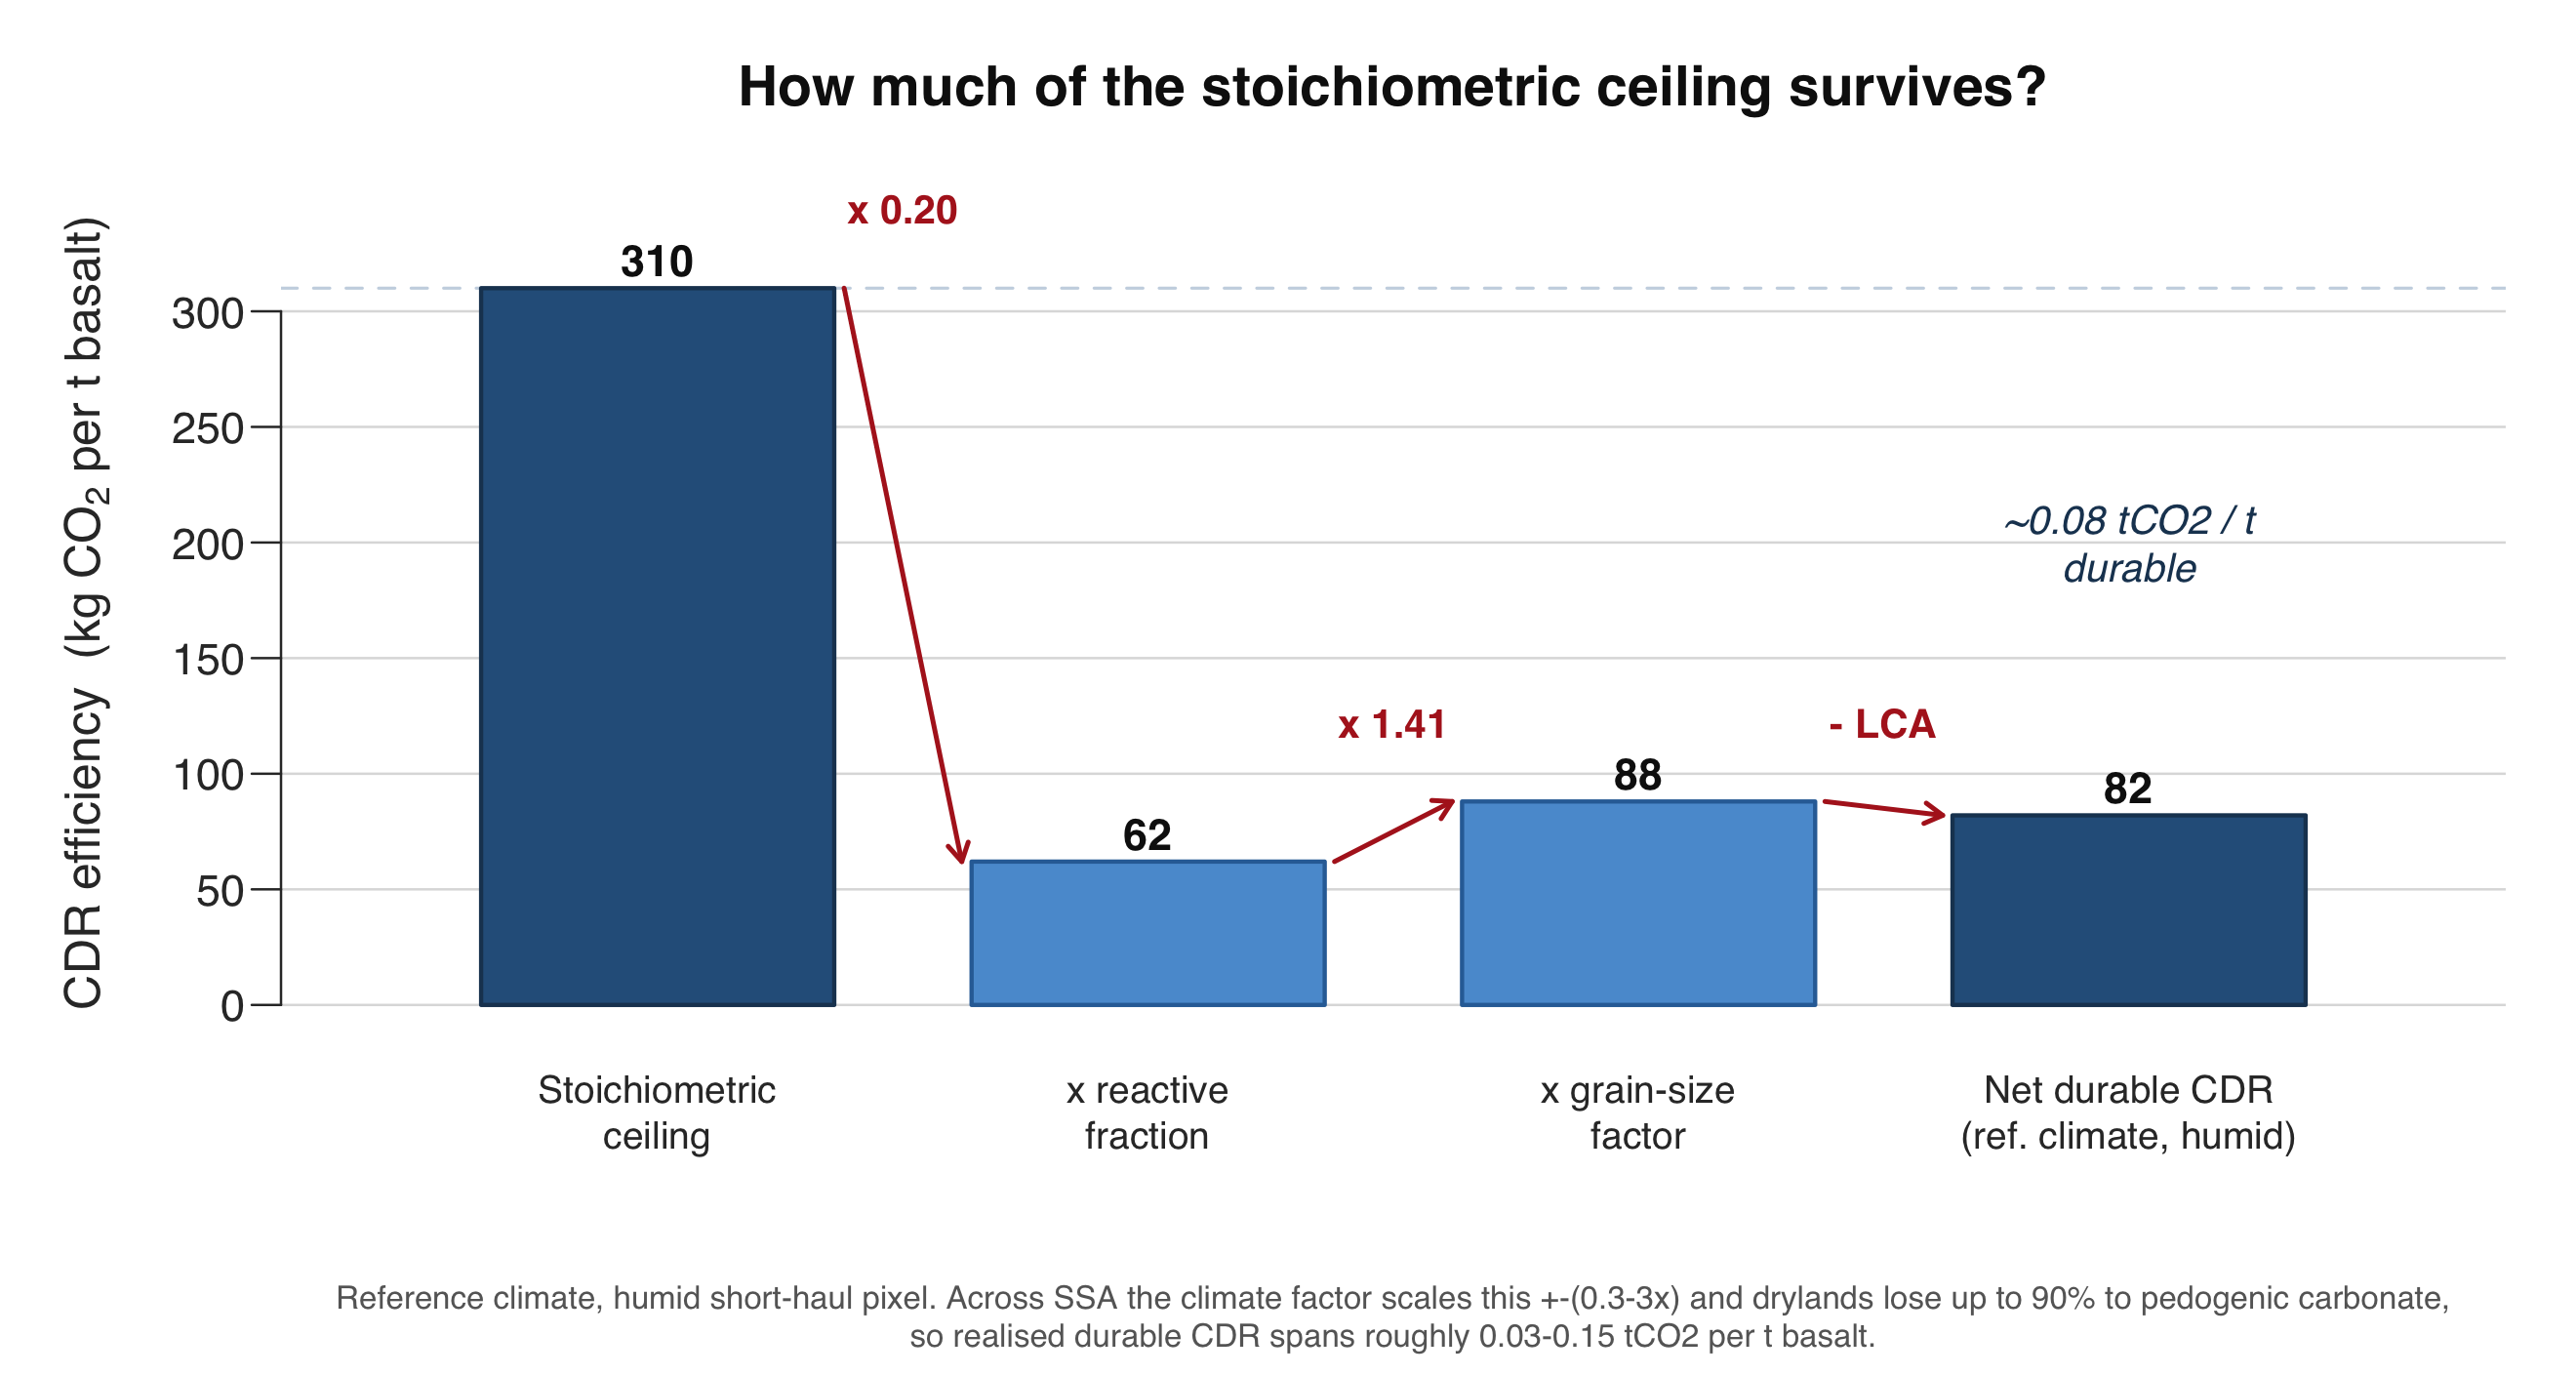
\includegraphics[width=0.86\linewidth]{figures/fig-cdr-cascade.png}
  \caption{How little of the stoichiometric ceiling survives. At a reference
  climate, humid, short-haul pixel the 310\,kg \co/t ceiling falls to
  $\sim$88\,kg gross and $\sim$82\,kg net of lifecycle emissions --- about
  0.08\,\tco\ per tonne of basalt. Across SSA the climate factor scales this
  by $0.3$--$3\times$ and drylands lose up to 90\% to pedogenic carbonate.}
  \label{fig:cascade}
\end{figure}

\section{The climate factor}

Dissolution speeds up with temperature and moisture and depends on pH. The model
uses interpretable multipliers, referenced to the US Corn Belt ($T_{\text{ref}}
= 11^{\circ}$C, $P_{\text{ref}} = 1000$\,mm) where the reactive fraction was
calibrated \citep{lewis2021}:
%
\begin{align}
f_{\text{MAT}} &= \mathrm{clamp}\!\left(\frac{\mathrm{MAT}}{11}, 0.3, 3.0\right),
\qquad
f_{\text{MAP}} = \mathrm{clamp}\!\left(\frac{\mathrm{MAP}}{1000}, 0.3, 3.0\right),
\label{eq:fmatmap}\\[2pt]
f_{\text{pH}} &=
\begin{cases}
0.5 & \mathrm{pH} < 4\\
0.5 + 0.5(\mathrm{pH}-4) & 4 \le \mathrm{pH} < 5\\
1.0 - 0.25(\mathrm{pH}-5) & 5 \le \mathrm{pH} < 7\\
0.5 & \mathrm{pH} \ge 7
\end{cases}
\label{eq:fph}\\[2pt]
f_{\text{climate}} &= f_{\text{MAT}}\cdot f_{\text{MAP}}\cdot f_{\text{pH}}.
\label{eq:fclimate}
\end{align}
%
The pH term (\autoref{eq:fph}) is triangular, peaking near pH 5 --- acid
catalysis is strongest on the acidic soils that also have the most agronomic
demand \citep{whitebrantley2003, brantley2008}. The effective reactive fraction
is then capped at unity,
%
\begin{equation}
\phi_{\text{eff}} = \min\!\big(1.0,\; \phi_0\, f_{\text{grain}}\,
f_{\text{climate}}\big),
\label{eq:phieff}
\end{equation}
%
and the per-tonne CDR at a pixel, before the net-export step, is
$\mathrm{CDR_{px}} = \mathrm{CDR_{max}}\cdot\phi_{\text{eff}}\cdot
(1-p_{\text{ped}})$.

\section{Pedogenic-carbonate loss}

In dry soils, some of the released calcium and magnesium re-precipitates as
secondary carbonate, re-releasing the captured \co. The lost fraction
$p_{\text{ped}}$ is binned by aridity (Aridity Index $=$ MAP/PET, from
\citealp{zomer2022}, with a MAP-only fallback), following the UNEP desertification
classes (\autoref{tbl:ped}). The exported fraction is $1-p_{\text{ped}}$.

\begin{longtable}[]{@{}lll@{}}
\caption{Pedogenic-carbonate loss fraction by aridity band
(\citealp{unep1992, renforth2019}).}\label{tbl:ped}\\
\toprule
Class & Aridity Index (MAP fallback) & $p_{\text{ped}}$ \\
\midrule
\endhead
Hyperarid & $<0.05$ ($<120$\,mm) & 0.90 \\
Arid & 0.05--0.20 (120--300\,mm) & 0.70 \\
Semi-arid & 0.20--0.50 (300--500\,mm) & 0.40 \\
Dry sub-humid & 0.50--0.65 (500--600\,mm) & 0.15 \\
Humid & $\ge 0.65$ ($\ge 600$\,mm) & 0.00 \\
\bottomrule
\end{longtable}

\section{Gross yield and the net-export correction}

Gross CDR per hectare is the rate times the per-tonne value,
$\mathrm{CDR_{gross}} = R \cdot \mathrm{CDR_{px}}/1000$ (\tco\,ha$^{-1}$,
cumulative over the horizon). But alkalinity that neutralises the soil's own
exchangeable acidity behaves exactly like lime: the carbon it captured is
re-released, so it is not \emph{durable} removal. The net-export correction
deducts this acidity sink first:
%
\begin{equation}
\mathrm{CDR_{net\text{-}export}}
= \max\!\big(0,\; \mathrm{CDR_{gross}} - F\cdot A\big),
\qquad F = \frac{\mathrm{CDR_{eff}}}{\mathrm{NV_{eff}}\cdot 1000} \approx 0.88,
\label{eq:netexport}
\end{equation}
%
where $A$ is the acidity sink expressed as CaCO$_3$-equivalent and $F\approx
0.88$ is the \co\ re-released per tonne of that lime-equivalent. This is a
first-order \emph{sequential bound} --- it assumes the acidity sink is filled
before any carbon is exported --- so the true durable CDR lies between
\autoref{eq:netexport} and the gross yield. Net-export is the recommended
default for the public/carbon case (\autoref{fig:netexport}).

\begin{figure}
  \centering
  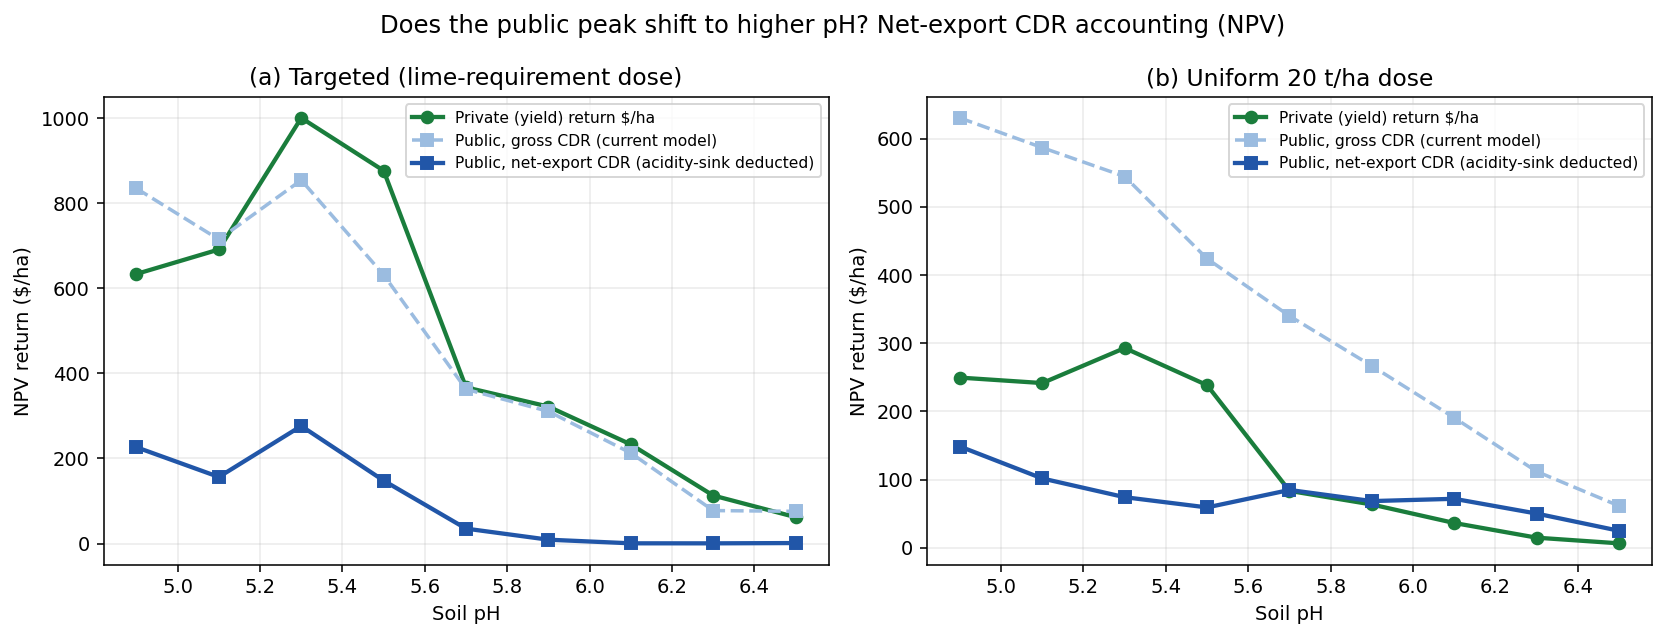
\includegraphics[width=\linewidth]{figures/fig-netexport.png}
  \caption{Gross vs.\ net-export CDR along the soil-pH gradient. On the most
  acidic soils (left), much of the alkalinity is consumed neutralising acidity,
  so durable (net-export) CDR is far below gross --- exactly where the private
  yield return is largest.}
  \label{fig:netexport}
\end{figure}

\begin{keybox}
\textbf{The load-bearing insight.} The private (yield) and public (durable CDR)
returns peak in \emph{different} places along the acidity gradient. Where soil
is very acidic, basalt's alkalinity is spent fixing the soil (great for yield,
little exported carbon); where soil is near-neutral, alkalinity is exported
(carbon) but there is little yield to gain. The two returns are spatially
complementary (\autoref{fig:schematic}).
\end{keybox}

\begin{figure}
  \centering
  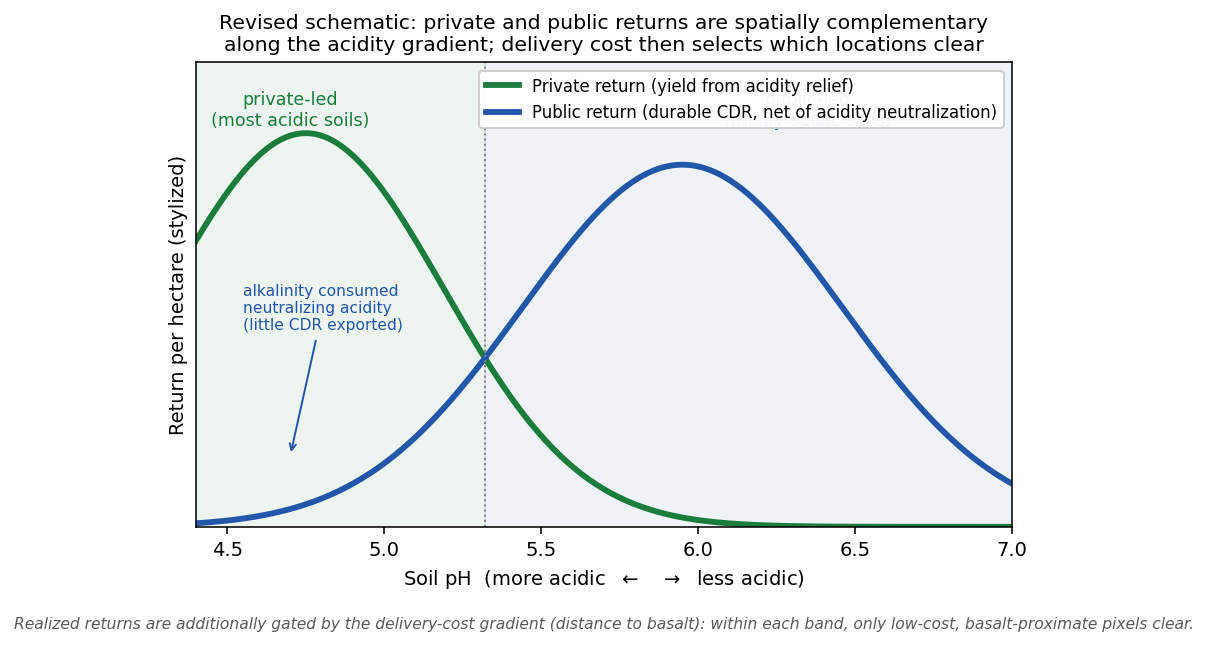
\includegraphics[width=0.9\linewidth]{figures/fig-schematic.png}
  \caption{Private and public returns are spatially complementary along the
  acidity gradient; delivery cost then selects which locations actually clear.}
  \label{fig:schematic}
\end{figure}

The spatial pattern of the CDR terms is shown in \autoref{fig:cdr-maps}. A full,
sourced derivation of every constant in this chapter is in the companion
\emph{CDR --- Technical Derivation}.

\begin{figure}
  \centering
  \begin{subfigure}{0.49\linewidth}
    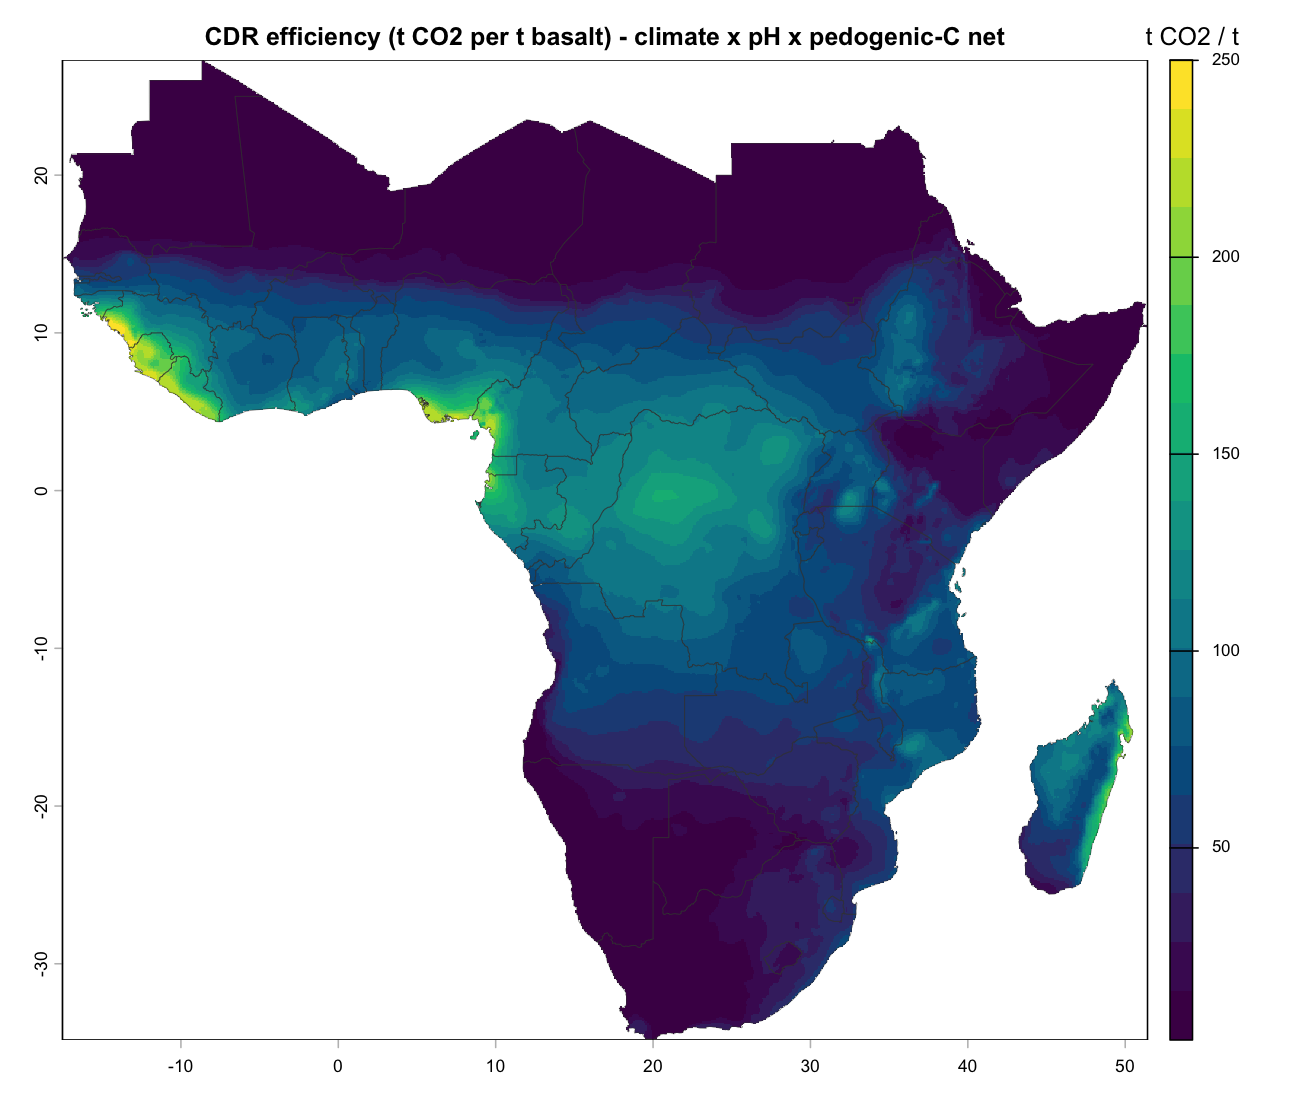
\includegraphics[width=\linewidth]{maps/03-cdr-per-t-basalt.png}
    \caption{Per-tonne CDR efficiency (\tco/t)}
  \end{subfigure}\hfill
  \begin{subfigure}{0.49\linewidth}
    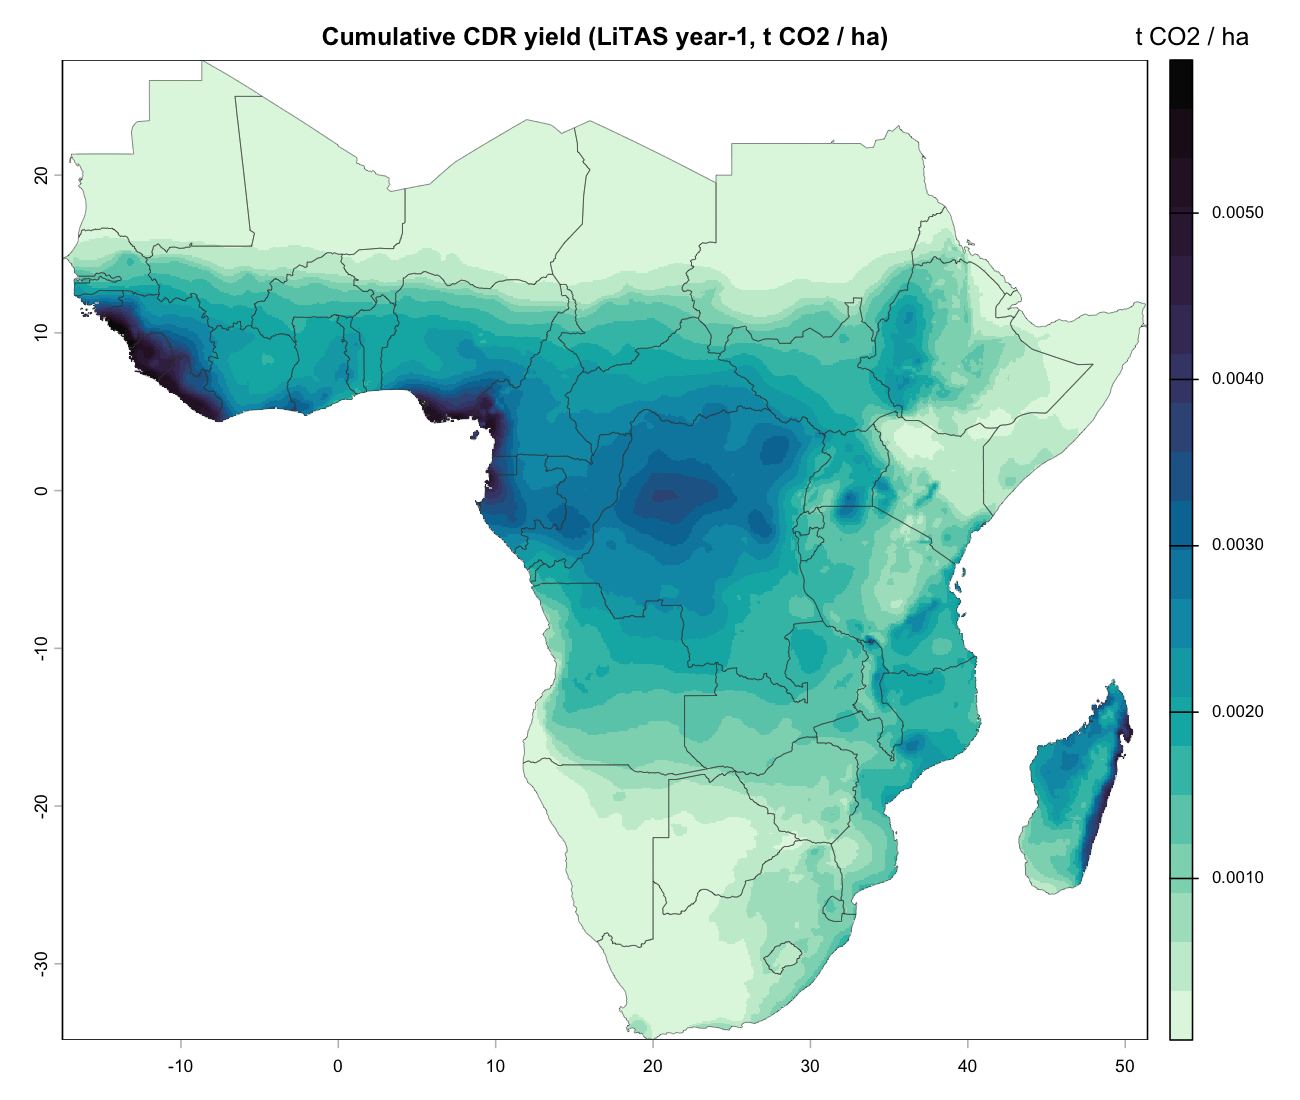
\includegraphics[width=\linewidth]{maps/04-cdr-yield-merlos.png}
    \caption{Cumulative CDR yield (\tco\,ha$^{-1}$)}
  \end{subfigure}
  \\[4pt]
  \begin{subfigure}{0.49\linewidth}
    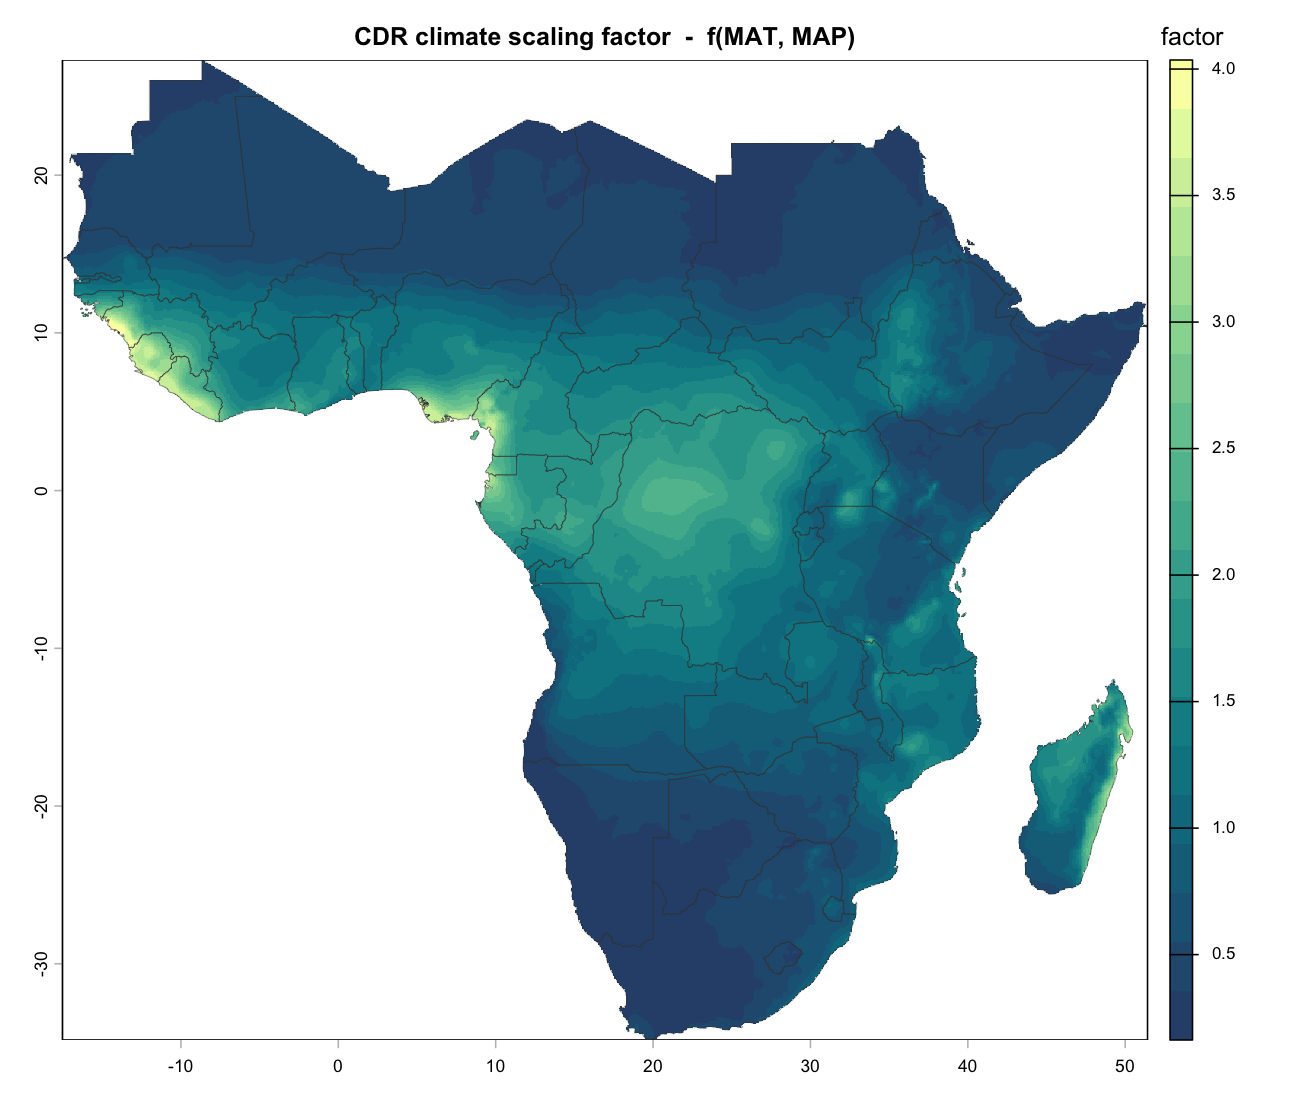
\includegraphics[width=\linewidth]{maps/05-cdr-climate-factor.png}
    \caption{Climate factor $f_{\text{climate}}$}
  \end{subfigure}\hfill
  \begin{subfigure}{0.49\linewidth}
    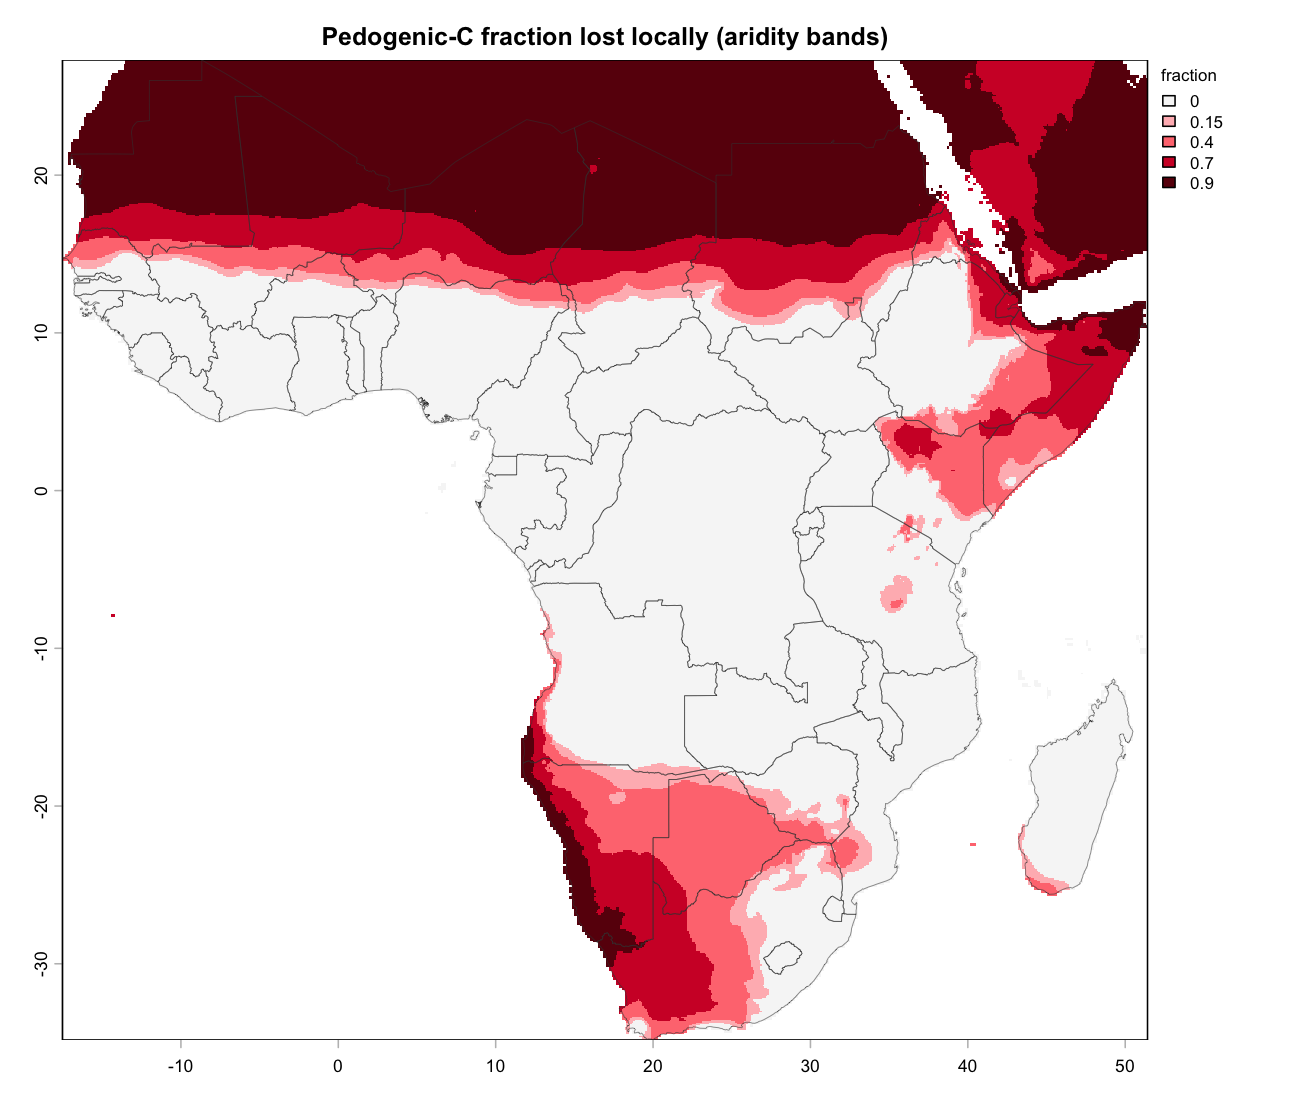
\includegraphics[width=\linewidth]{maps/06-pedogenic-fraction.png}
    \caption{Pedogenic-loss fraction $p_{\text{ped}}$}
  \end{subfigure}
  \caption{The CDR surface and its two spatial modifiers.}
  \label{fig:cdr-maps}
\end{figure}

% ==================================================================
\chapter{Crop response: the agronomic stream}\label{ch:crop}

The agronomic return is the yield uplift a farmer captures when basalt relieves
soil acidity, valued at the local producer price. The model offers two ways to
estimate that uplift: a deterministic \emph{EcoCrop} suitability model (the
default) and an optional trial-anchored \emph{Bayesian} model.

\section{EcoCrop, conceptually}

EcoCrop scores how suitable an environmental condition is for a crop on a
0--1 scale, using a piecewise-linear \emph{tolerance envelope} --- a trapezoid
with four breakpoints: an absolute minimum below which suitability is zero, an
optimal band where it is one, and an absolute maximum above which it is zero
again (\autoref{fig:ecocrop}a). It is a decades-old agronomic standard,
implemented in R as \texttt{Recocrop} \citep{recocrop}.

\begin{figure}
  \centering
  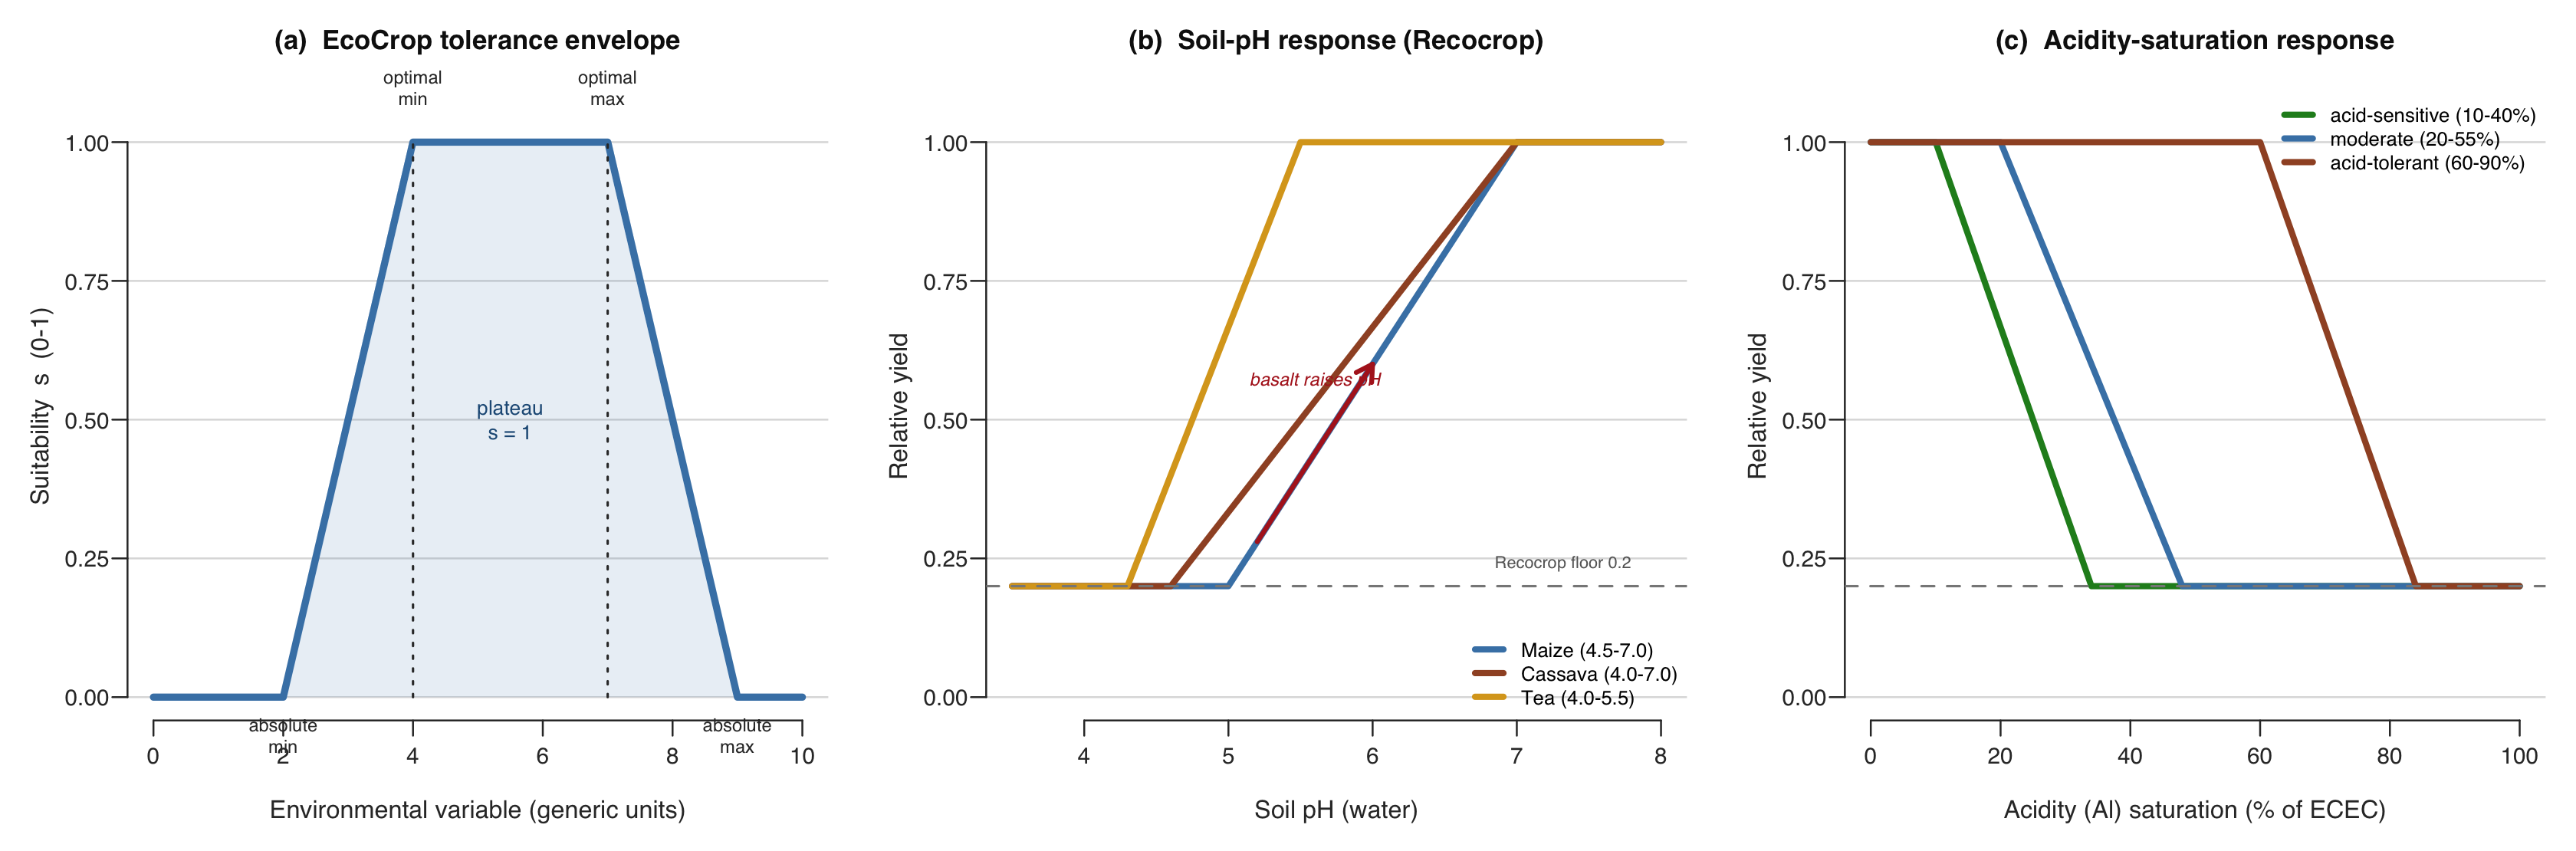
\includegraphics[width=\linewidth]{figures/fig-ecocrop-concept.png}
  \caption{The EcoCrop suitability model. (a) The generic trapezoidal tolerance
  envelope with its four breakpoints. (b) The soil-pH response as parameterised
  in this pipeline --- relative yield rises from a floor to a plateau across each
  crop's $[\text{min\_ph},\text{max\_ph}]$ band; the red arrow shows how basalt,
  by raising pH, moves an acidic soil up its curve. (c) The acidity-saturation
  response --- a plateau to the crop's tolerance, then a linear decline. Both
  are clamped to a floor of 0.2.}
  \label{fig:ecocrop}
\end{figure}

The key modelling insight is that the yield response to soil acidity is the same
whether the amendment is lime or basalt --- so a pH/acidity suitability model is
a legitimate proxy for basalt's agronomic uplift. In this pipeline the envelope
is parameterised two ways per crop:
%
\begin{itemize}
\item \textbf{Soil-pH response} (\autoref{fig:ecocrop}b): relative yield is a
floor below the crop's \texttt{min\_ph}, rises linearly to 1 at
\texttt{max\_ph}, and plateaus above. Acid-loving crops have low upper bounds
(tea 5.5, cocoa 6.0, coffee 6.5); cereals and legumes 7.0--8.0.
\item \textbf{Acidity-saturation response} (\autoref{fig:ecocrop}c): relative
yield is 1 up to the crop's aluminium-saturation tolerance \texttt{ac\_sat}
(\% of ECEC), then declines linearly to 0 at \texttt{max\_ac\_sat}.
\end{itemize}
%
Every raster is clamped to $[0.2, 1]$: no pixel is assigned less than 20\% of
attainable yield. \texttt{erw-5} evaluates these envelopes on the soil stack via
\texttt{Recocrop::ecocrop} to produce 46 rasters (23 crops $\times$ 2 responses).

\begin{keybox}
\textbf{A modelling choice that unlocked most of SSA.} An earlier version used a
flat upper pH bound of 5.5 for \emph{every} crop, which zeroed the agronomic
credit across the pH 5.5--7.0 belt that covers most SSA savanna and Sahel.
Replacing it with per-crop EcoCrop optima (5.5--8.0) restored a non-zero yield
response on that belt --- one of the single largest drivers of the refreshed
results (\autoref{ch:results}).
\end{keybox}

\section{From suitability to revenue}

Inside the profitability engine (\texttt{erw-7}) the EcoCrop relative-yield
raster $\text{loss}\in[0.2,1]$ is converted to a recoverable tonnage response by
dividing the actual yield by the suitability and taking the shortfall,
%
\begin{equation}
\Delta Y = \frac{Y_0}{\text{loss}} - Y_0,
\qquad R_{\mathrm{agro}} = \Delta Y \times p_c,
\label{eq:agro}
\end{equation}
%
with $p_c$ the FAOSTAT producer price. The uplift is largest where the soil is
acidic \emph{and} the crop is acid-sensitive; it is near zero on already-neutral
soils and for acid-tolerant crops (cassava, sorghum, millet), whose response is
effectively saturated --- which is why those crops must clear the full basalt
cost on carbon revenue alone.

\section{The Bayesian arm (optional, not run at v1)}

Where a trial-anchored estimate is preferred, \texttt{erw-yield-fit} fits a
Bayesian multilevel meta-regression of the log yield-ratio (basalt vs.\ control)
on ERW covariates, with per-observation known measurement error and crossed
crop/site random intercepts \citep{burkner2017}:
%
\begin{equation}
\begin{split}
\log\!\left(\frac{Y_{\text{treat}}}{Y_{\text{control}}}\right)_i \Big| \mathrm{se}_i
&\sim \beta_0 + \beta_1\log \text{rate} + \beta_2\,\mathrm{pH}
+ \beta_3\,\mathrm{MAT} \\
&\quad + \beta_4\,\mathrm{MAP} + \beta_5\log \text{grain}
+ \alpha_{\text{crop}} + \alpha_{\text{site}} + \varepsilon_i.
\end{split}
\label{eq:bayes}
\end{equation}
%
\texttt{erw-yield-predict} then maps the posterior-mean coefficients over the
per-pixel covariates to a yield-ratio uplift raster, which \texttt{erw-7}
prefers over EcoCrop when present. At v1 the trial table has only $\sim$14 rows,
so the fit is prior-dominated: the framework is in place but the arm is
\textbf{not run}, and EcoCrop is the operative response.

% ==================================================================
\chapter{Cost, logistics, and energy}\label{ch:cost}

The cost stream builds the delivered-and-applied price of basalt pixel by pixel,
and --- because grinding and haulage burn diesel and electricity --- the
lifecycle emissions that must be netted off the gross CDR.

\section{Feedstock supply and logistics (B4)}

Basalt sources are the basic-volcanic, pyroclastic, and gabbro classes of the
GLiM lithological map \citep{hartmann2012}; ultramafics are excluded for their
nickel/chromium leaching risk. From every cropland pixel, \texttt{terra::costDist}
computes the least-cost travel time to the nearest source over the Malaria Atlas
motorised friction surface \citep{weiss2020}. Travel time becomes distance and
cost through simple, transparent constants (\autoref{tbl:logistics}):
%
\begin{align}
C_{\text{transport}} &= t_{\text{travel}} \times 0.04\ \text{\$/min/t},
\qquad
d_{\text{km}} = t_{\text{travel}} \times 0.5, \label{eq:transport}\\
C_{\text{bas/t}} &= \underbrace{10}_{\text{quarry}}
 + \underbrace{C_{\text{grind}}}_{\text{energy}}
 + C_{\text{transport}}
 + \underbrace{8}_{\text{spreading}}\quad(\text{\$/t}). \label{eq:cbas}
\end{align}
%
Haulage is capped at 1000\,km, beyond which diesel emissions would erase the
credit and cost makes basalt uncompetitive with lime. The delivered price
surface is shown in \autoref{fig:cost-maps}.

\begin{longtable}[]{@{}lll@{}}
\caption{Logistics and cost constants.}\label{tbl:logistics}\\
\toprule
Constant & Value & Note \\
\midrule
\endhead
Quarry-gate price & \$10/t & Ex-quarry basalt fines \\
Truck haulage & \$0.04/min/t & 30-t truck at \$80/hr \\
Effective speed & 0.5\,km/min & $\approx$30\,km/h on-friction \\
Max haul & 1000\,km & Beyond this, unreachable \\
Spreading & \$8/t & On-farm application \\
Grinding (50\,\um) & 19.4\,kWh/t & \autoref{eq:grind} \\
Truck emissions & 0.12\,kg\,\co/t/km & Diesel LCA \\
Spreading emissions & 0.5\,kg\,\co/t & $\approx$0.1\,L diesel/t \\
\bottomrule
\end{longtable}

\section{Energy: the largest lifecycle lever (B5)}

Grinding cost and grinding emissions are both local: the same 19.4\,kWh/t is
priced at the country's industrial electricity tariff and emits at the country's
grid carbon intensity. \texttt{erw-energy-country} rasterises a 43-country table.
The grid carbon intensity spans roughly \textbf{0.03\,kg\,\co/kWh} (hydro-rich
Ethiopia, DR Congo) to \textbf{0.95\,kg\,\co/kWh} (coal-based South Africa) --- a
$\sim$30$\times$ spread that makes electricity, not any weathering parameter, the
single largest control on \emph{lifecycle} emissions.

\section{Lifecycle emissions}

Per tonne of basalt, lifecycle emissions sum grinding, transport, and spreading:
%
\begin{equation}
L = \underbrace{(\text{kWh/t})\cdot \mathrm{CI}}_{\text{grinding}}
  + \underbrace{d_{\text{km}}\cdot 0.12}_{\text{transport}}
  + \underbrace{0.5}_{\text{spreading}}
  \quad(\text{kg \co/t}),
\label{eq:lca}
\end{equation}
%
with $\mathrm{CI}$ the grid carbon intensity. This $L$ is what the profitability
engine deducts from gross CDR to get the net removal that earns credits.

\begin{figure}
  \centering
  \begin{subfigure}{0.49\linewidth}
    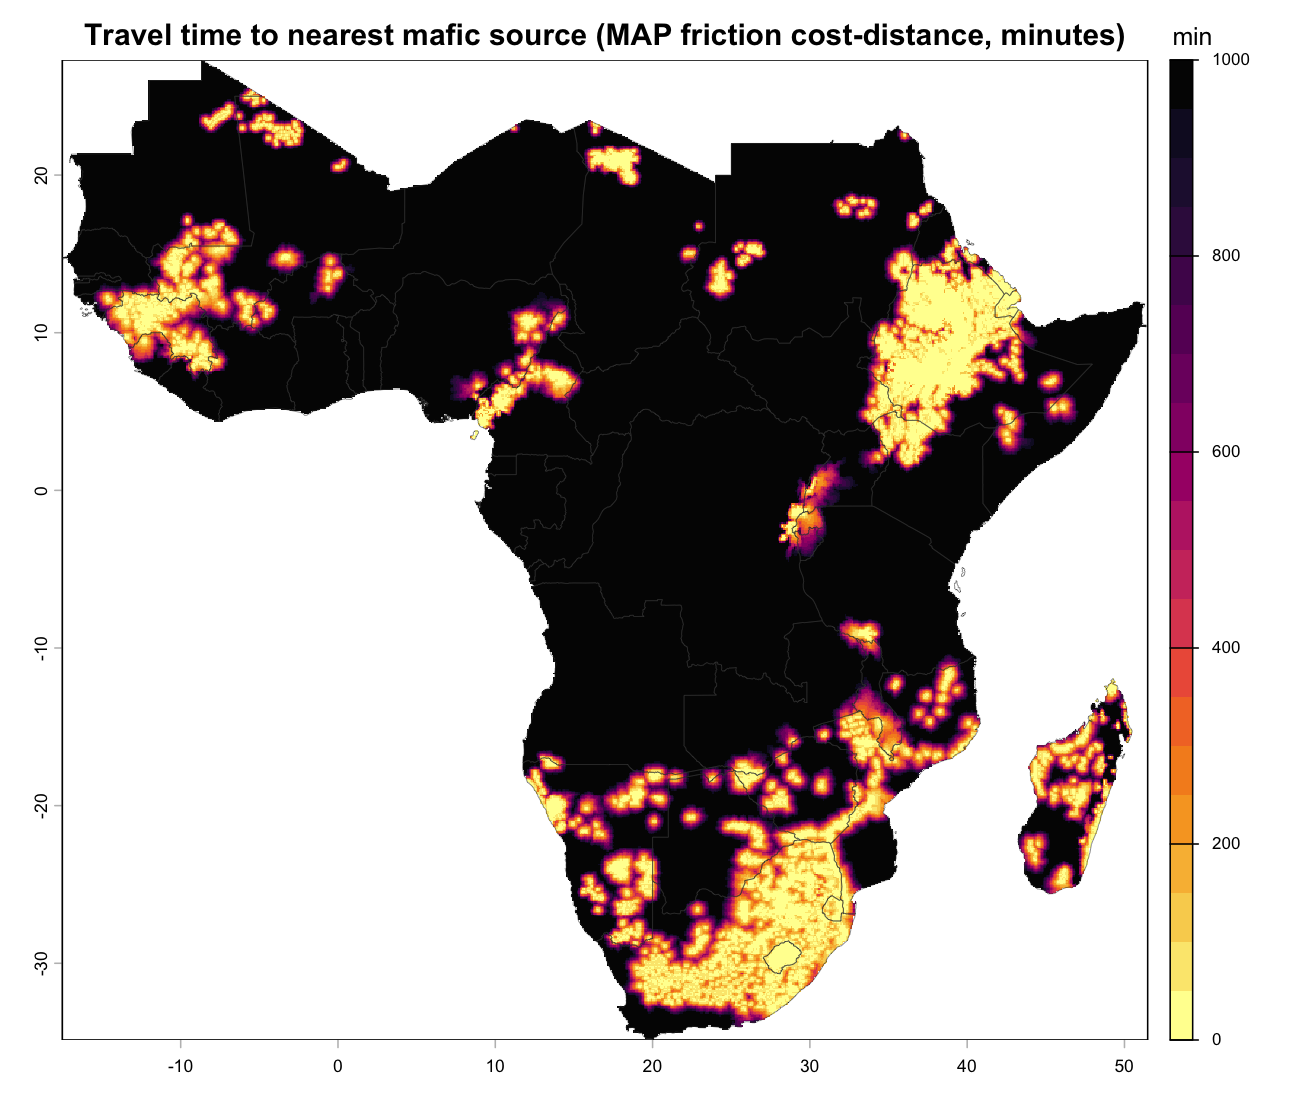
\includegraphics[width=\linewidth]{maps/10-basalt-traveltime.png}
    \caption{Travel time to nearest source (min)}
  \end{subfigure}\hfill
  \begin{subfigure}{0.49\linewidth}
    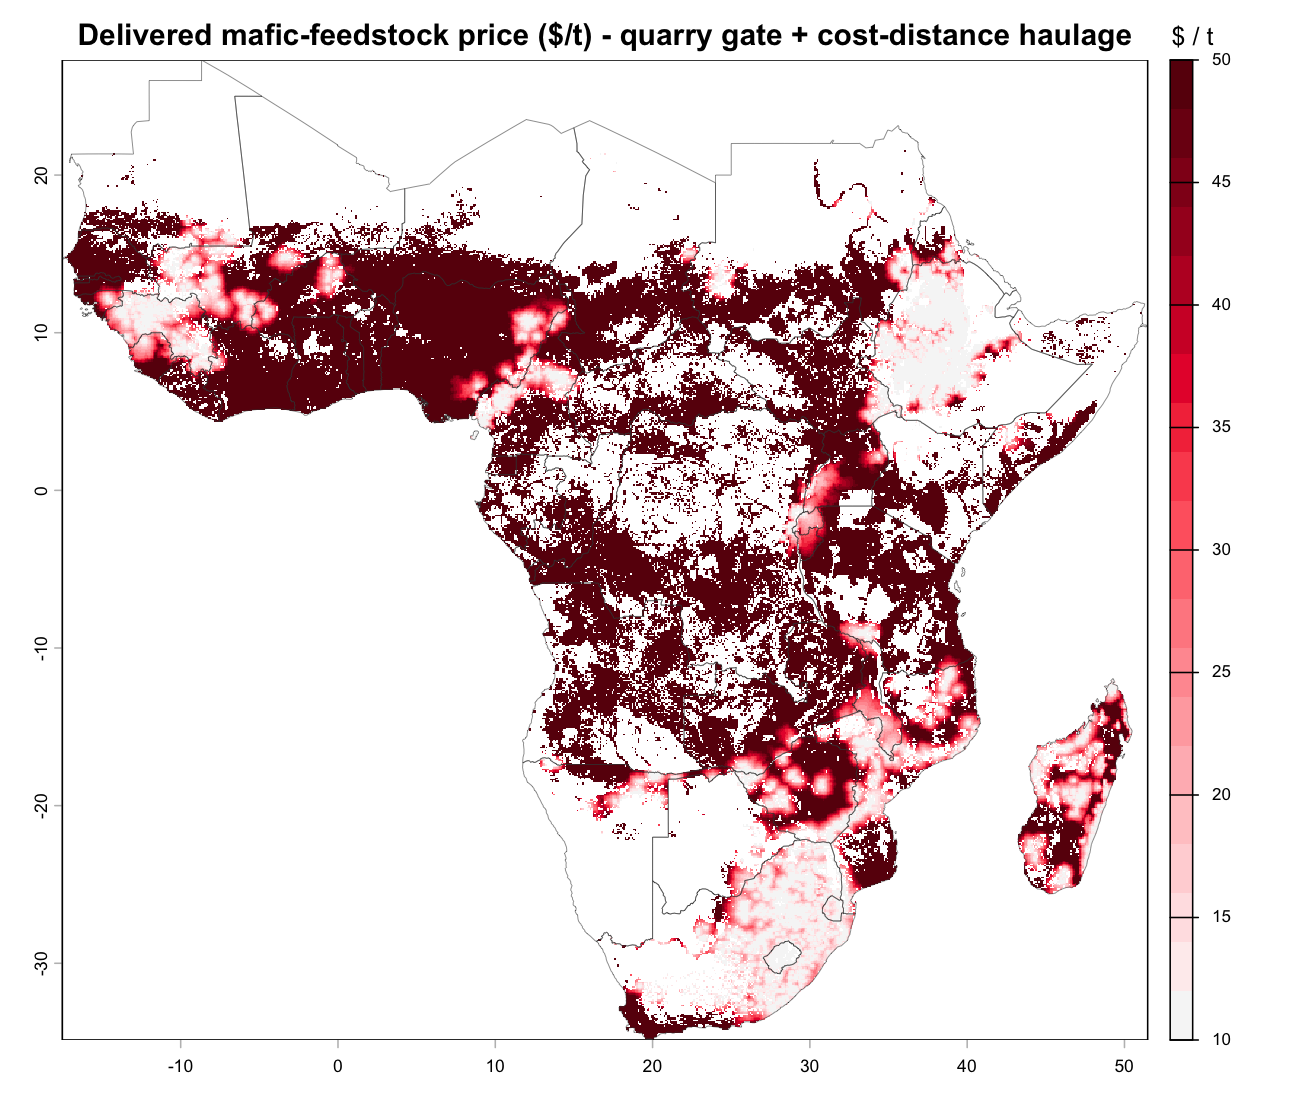
\includegraphics[width=\linewidth]{maps/11-basalt-delivered-price.png}
    \caption{Delivered basalt price (\$/t)}
  \end{subfigure}
  \caption{Logistics surfaces. Delivered price is lowest near basalt outcrops
  and rises with haul distance; it is the gate that decides which otherwise
  profitable pixels actually clear.}
  \label{fig:cost-maps}
\end{figure}

% ==================================================================
\chapter{Profitability}\label{ch:profit}

The profitability engine (\texttt{erw-7}) assembles the three streams into
\autoref{eq:master} for every crop, allocation, and regime --- 276 output
rasters in all.

\section{The gross-margin identity, concretely}

\begin{align}
\mathrm{Rev_{CDR}} &= \mathrm{CDR_{net}}\times(p_{\co} - \mathrm{MRV}),
  \label{eq:revcdr}\\
\mathrm{CDR_{net}} &= \max\!\big(0,\ \mathrm{CDR_{gross}} - R\,L/1000\big),\\
\mathrm{Rev_{agro}} &= \Delta Y \times p_c,\qquad
  C_{\text{basalt}} = R \times C_{\text{bas/t}}, \label{eq:revagro}\\
\mathrm{GM_{combined}} &= \mathrm{Rev_{agro}} + \mathrm{Rev_{CDR}}
  - C_{\text{basalt}}. \label{eq:gm}
\end{align}
%
The engine also reports agro-only and CDR-only margins and a return-on-investment
$\mathrm{ROI} = (\mathrm{Rev_{agro}}+\mathrm{Rev_{CDR}})/C_{\text{basalt}}$.
Default economic constants are in \autoref{tbl:econ}.

\begin{longtable}[]{@{}lll@{}}
\caption{Default economic and carbon-market constants (\texttt{erw-7}).}\label{tbl:econ}\\
\toprule
Constant & Value & Source \\
\midrule
\endhead
Carbon price $p_{\co}$ & \$150/\tco & VCM mid 2024--25 \citep{levy2024} \\
MRV cost & \$20/\tco & \citet{levy2024} \\
Discount rate & 10\% & Conventional \\
Project horizon & 5\,yr & Accreditation window \\
CDR phasing & 0.30/0.25/0.20/0.15/0.10 & \citet{kanzaki2023} \\
Grid CI fallback & 0.60\,kg/kWh & \citet{ipcc2019} \\
\bottomrule
\end{longtable}

\section{Three temporal accounting regimes}

The same pixel can be scored three ways, reflecting genuinely different questions
about \emph{when} the returns land (\autoref{tbl:regimes}).

\begin{longtable}[]{@{}lp{9.2cm}@{}}
\caption{The three return regimes.}\label{tbl:regimes}\\
\toprule
Regime & Definition \\
\midrule
\endhead
\texttt{year1} & One application; agronomic return accumulated
\emph{undiscounted} over the 5-year residency to match the horizon-cumulative
CDR: $\mathrm{GM} = \mathrm{Rev_{agro}}\times 5 + \mathrm{Rev_{CDR}} -
C_{\text{basalt}}$. \\
\texttt{npv} & Agronomic return discounted at 10\% over the reapplication
interval (via \texttt{limer::NPV\_lime}); CDR revenue multiplied by the CDR-NPV
factor $\approx 0.79$. \\
\texttt{equilibrium} & Steady state: the annual \emph{maintenance} rate and its
CDR, no horizon multiplier and no discount factor. \\
\bottomrule
\end{longtable}

The CDR-NPV factor discounts the phased removal relative to treating it as
upfront:
%
\begin{equation}
\text{CDR-NPV factor} = \frac{\sum_{t} f_t/(1+r)^{t}}{\sum_{t} f_t}
\approx 0.79,
\label{eq:npvfactor}
\end{equation}
%
with $r = 10\%$ and the phasing $f=\{0.30,0.25,0.20,0.15,0.10\}$.

\section{Allocation rules and breakeven carbon price}

Four allocation rules are scored: \texttt{targeted} (the LiTAS dose, only on
pixels acidic beyond each crop's tolerance) and \texttt{uniform\_10/20/50}. The
targeted rule is the parsimonious one --- it applies basalt only where the soil
actually needs it --- while the uniform rules mirror the continental-study
convention and expose the over-application penalty (\autoref{ch:supply}).

Rearranging \autoref{eq:gm} for the carbon price that drives the crop-weighted
margin to zero gives the \emph{breakeven carbon price}, a map of how high the
carbon market must be for ERW to clear at each location:
%
\begin{equation}
p_{\co}^{\text{breakeven}} =
\frac{C_{\text{basalt}} - \mathrm{Rev_{agro}}}{\mathrm{CDR_{net}}} + \mathrm{MRV}.
\label{eq:breakeven}
\end{equation}
%
\autoref{fig:profit-maps} shows the year-1 targeted gross margin and its
breakeven surface.

\begin{figure}
  \centering
  \begin{subfigure}{0.49\linewidth}
    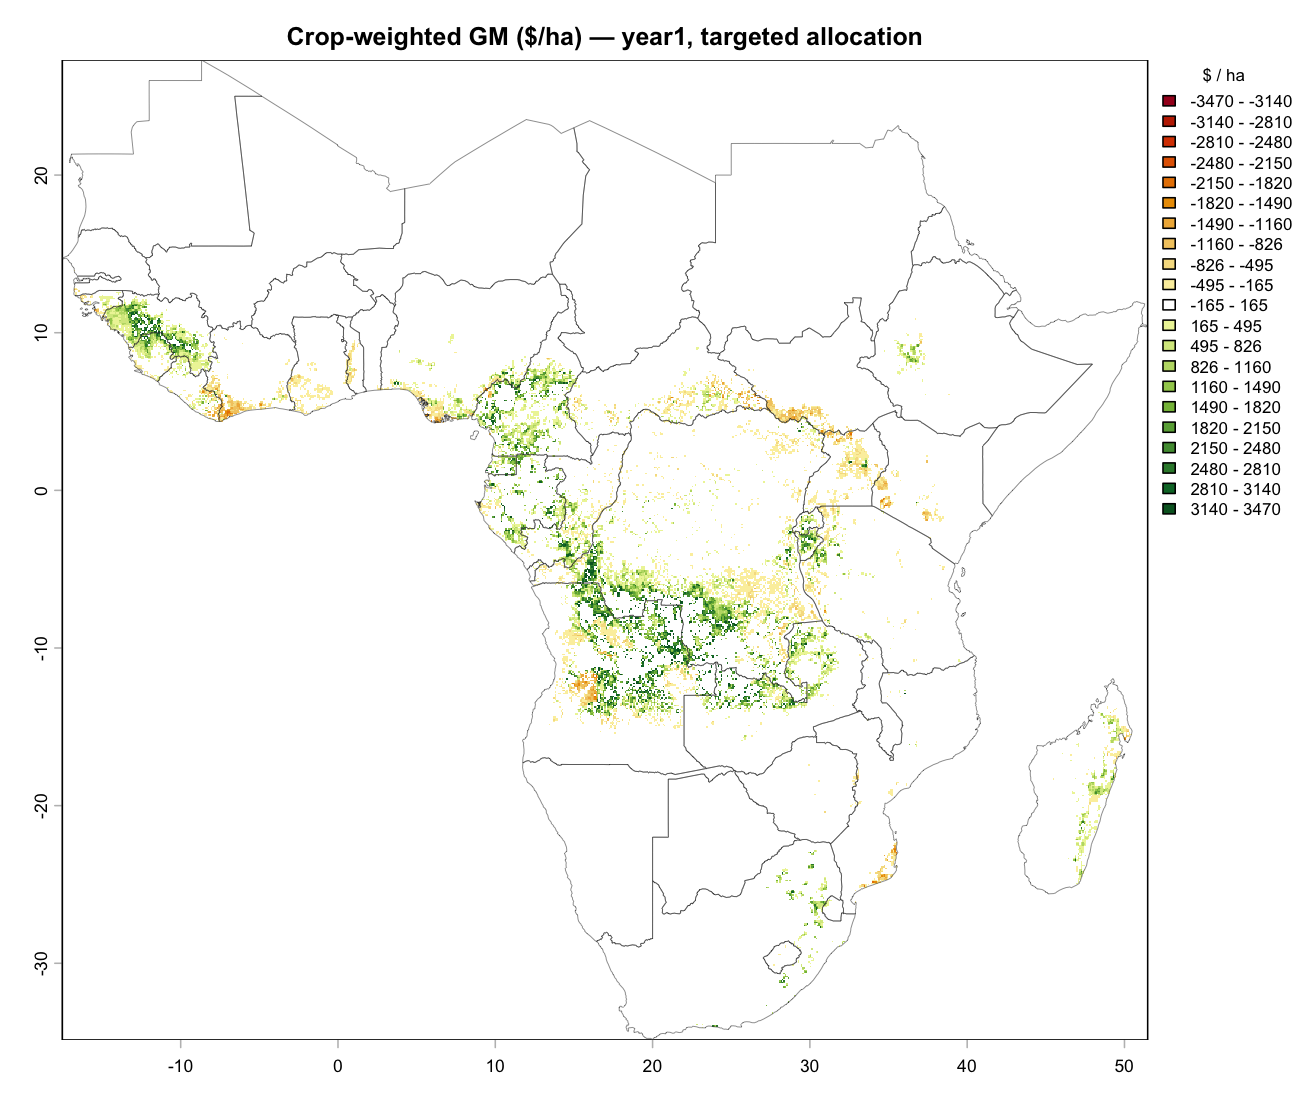
\includegraphics[width=\linewidth]{maps/profitability/ssa_gm_year1_targeted.png}
    \caption{Crop-weighted gross margin (\$/ha)}
  \end{subfigure}\hfill
  \begin{subfigure}{0.49\linewidth}
    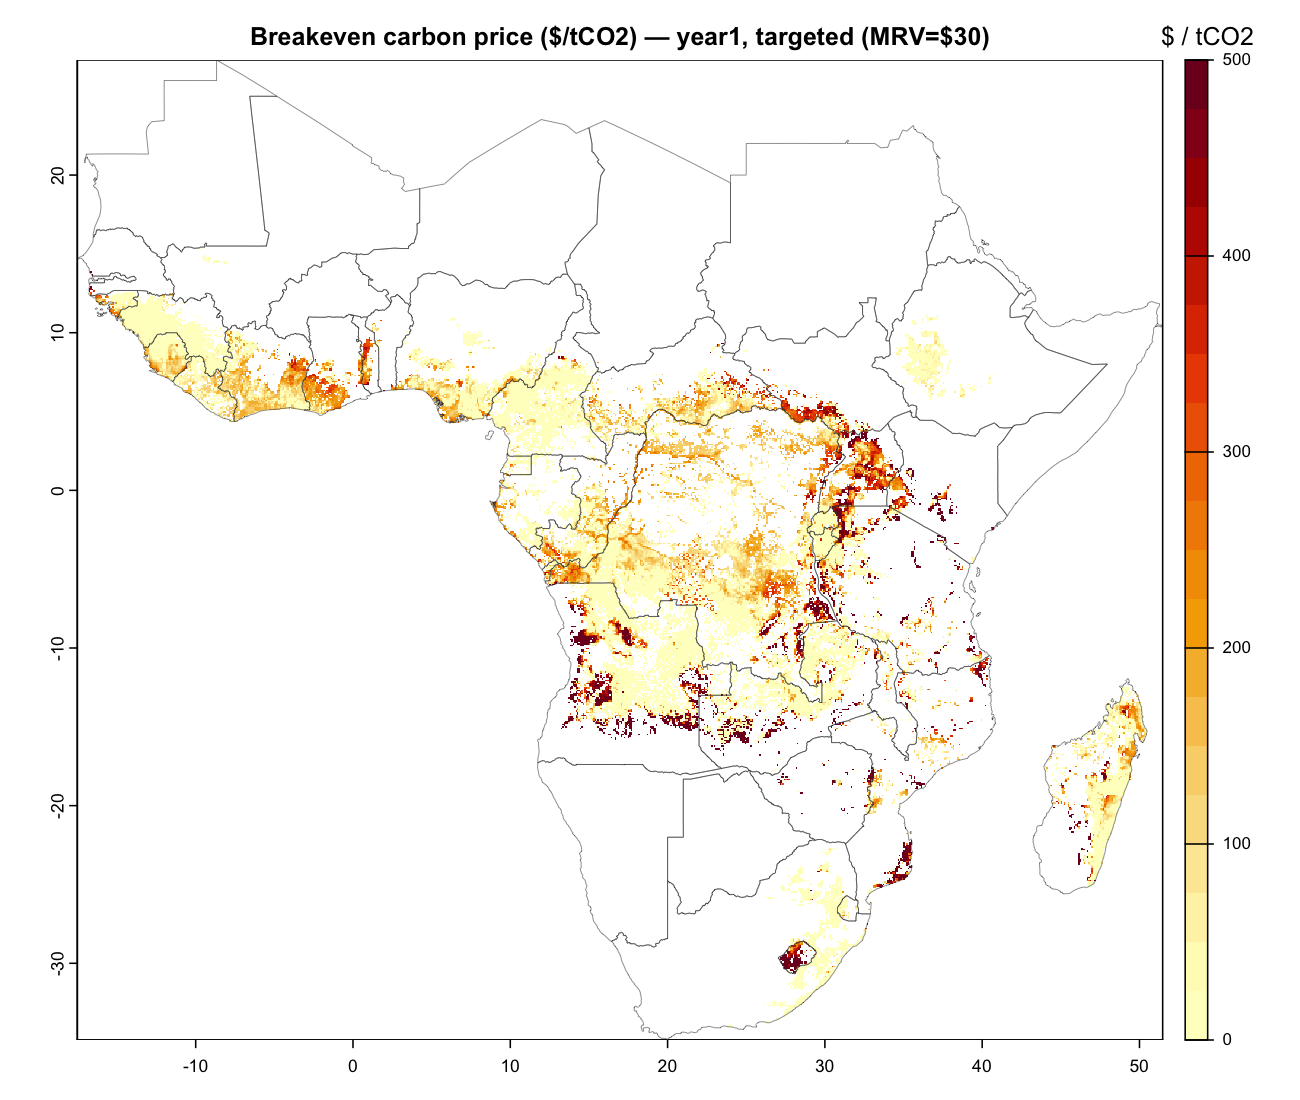
\includegraphics[width=\linewidth]{maps/profitability/breakeven_carbon_year1_targeted.png}
    \caption{Breakeven carbon price (\$/\tco)}
  \end{subfigure}
  \caption{Profitability outcome maps, year-1 targeted allocation.}
  \label{fig:profit-maps}
\end{figure}

\begin{keybox}
\textbf{Worked intuition (pre-refresh defaults, for teaching).} Pixel A near
Kisumu, Kenya (pH 5.2, warm and wet, 150\,km haul) reaches
$\mathrm{CDR_{px}}\approx 172$\,kg/t and $\sim$4.6\,\tco/ha net; Pixel B near
Kaya, Burkina Faso (pH 6.0, semi-arid, 500\,km haul) reaches only
$\sim$58\,kg/t --- and there the lifecycle emissions exceed the gross capture, so
net CDR is zero. The lesson: basalt cost dominates, climate is the second-largest
lever, and \emph{which pixel} you pick matters more than the average price.
\end{keybox}

% ==================================================================
\chapter{Supply curves and sensitivity}\label{ch:supply}

\section{Supply ranking (B8)}

When basalt supply is the scarce input, the right way to deploy a limited annual
tonnage is to rank pixels by \emph{gross margin per tonne of basalt} --- the
shadow value of the supply constraint --- and fill from the top until the cap
binds. \texttt{erw-supply} does exactly this, producing a supply curve of
marginal \$/t basalt against annual capacity and the cumulative carbon it buys.

\begin{keybox}
\textbf{Ranking and cap matter as much as parameters.} Because the profitable
pixels are a minority of a heavy-tailed distribution, a well-chosen top decile is
strongly positive even where the SSA-wide \emph{mean} is negative. The deployment
question is therefore ``which pixels, up to what cap?'' at least as much as ``what
carbon price?''.
\end{keybox}

\section{Kinetic saturation makes CDR concave in dose}

Applying more basalt does not buy proportionally more durable carbon: the soil's
acidity sink is filled first (\autoref{eq:netexport}), and the reactive fraction
saturates. Durable net-export CDR is therefore concave --- even non-monotone ---
in the application rate (\autoref{fig:saturation}), which is precisely why the
uniform-50 rule destroys value.

\begin{figure}
  \centering
  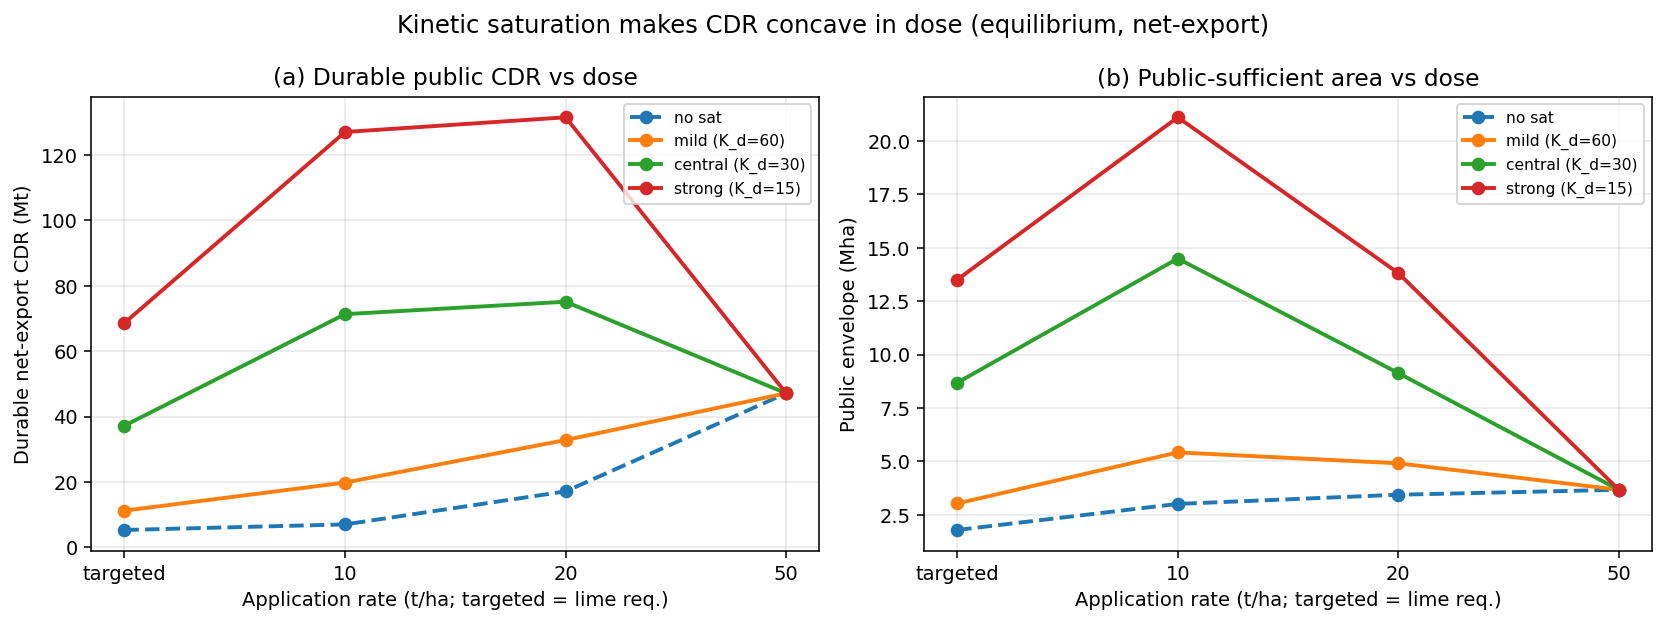
\includegraphics[width=\linewidth]{figures/fig-saturation.png}
  \caption{Kinetic saturation: durable public CDR and the public-sufficient area
  are concave in dose. Past a point, extra basalt adds cost and lifecycle
  emissions faster than durable removal.}
  \label{fig:saturation}
\end{figure}

\section{Sensitivity sweeps (B9)}

\texttt{erw-8} runs five one- or two-dimensional sweeps over the whole engine,
across all three regimes and 23 crops (\autoref{tbl:sweeps}).

\begin{longtable}[]{@{}l>{\raggedright\arraybackslash}p{10.4cm}@{}}
\caption{Sensitivity sweeps.}\label{tbl:sweeps}\\
\toprule
Sweep & Grid \\
\midrule
\endhead
Prices & crop $\times$ basalt price multipliers $\{0.5\ldots2.0\}$,
carbon $\{0,50,100,150,250\}$ \\
Yields & yield-gap factor $\{1.0,1.25,\ldots,2.5\}$ \\
MRV & $\{0,15,30,50,80\}$\,\$/\tco \\
Grain & $\{10,30,50,100,200,500\}$\,\um\ (reactivity vs.\ grinding) \\
Allocation & targeted, uniform 10/20/50 \\
\bottomrule
\end{longtable}

The over-application penalty is visible in \autoref{fig:overliming}: private
return falls steadily from the targeted (lime-requirement) dose through the
uniform ladder, and the over-liming sensitivity band widens as the dose grows.

\begin{figure}
  \centering
  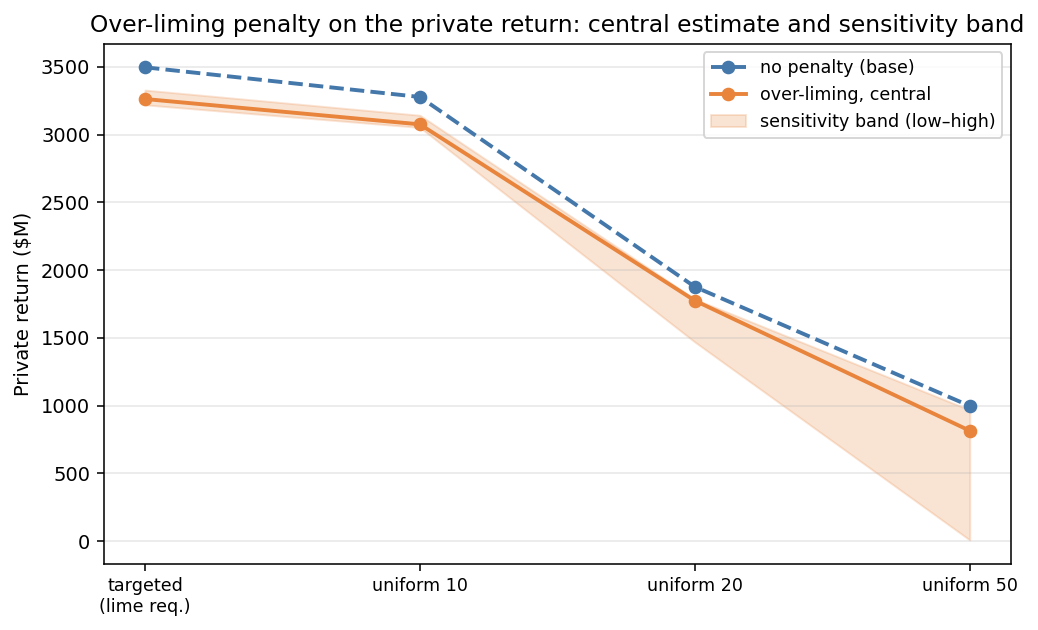
\includegraphics[width=0.86\linewidth]{figures/fig-overliming.png}
  \caption{Over-application penalty on the private return across allocation
  rules. The targeted (lime-requirement) dose dominates; uniform-50 gives up
  most of the value.}
  \label{fig:overliming}
\end{figure}

\section{Private, public, and combined returns}\label{sec:envelopes-method}

A dedicated analysis (\texttt{erw-11}) asks a sharper question than ``is the pixel
profitable?'': \emph{which} of the two returns carries it. Because \texttt{erw-7}
already separates the agronomic and CDR margins --- each measured against the
\emph{full} delivered basalt cost --- every pixel can be classified by three
independent sufficiency tests:
%
\begin{align}
\text{private-sufficient} &\iff
  \mathrm{GM_{agro\text{-}only}} = R_{\mathrm{agro}} - C_{\text{basalt}} > 0,
  \label{eq:privsuf}\\
\text{public-sufficient} &\iff
  \mathrm{GM_{CDR\text{-}only}} = R_{\mathrm{CDR}} - C_{\text{basalt}} > 0,
  \label{eq:pubsuf}\\
\text{combined-sufficient} &\iff
  \mathrm{GM_{combined}} = R_{\mathrm{agro}} + R_{\mathrm{CDR}}
  - C_{\text{basalt}} > 0. \label{eq:combsuf}
\end{align}
%
Private-sufficient land pays for itself on yield alone --- a grower would invest
with or without carbon finance; public-sufficient land pays on carbon revenue
alone --- a buyer would fund it with or without yield gains. Their
\emph{intersection} is doubly justified and, crucially, is exactly where carbon
credits are \emph{least additional}, because the agronomic case already stands on
its own. This yields a five-way per-pixel typology: \textbf{both},
\textbf{private-only}, \textbf{public-only}, \textbf{combined-only} (neither
stream alone suffices but stacked they do), and \textbf{neither}.

\subsection{Robustness and the core targeting area}

Because the intersection is parameter-sensitive, \texttt{erw-11} recomputes it
analytically over a 240-point grid --- delivered cost $\times\{0.5\text{--}2.0\}$,
carbon price $\{\$50\text{--}250\}$, yield $\times\{0.5\text{--}2.0\}$, CDR rate
$\times\{0.5\text{--}1.5\}$ --- and scores each pixel by the fraction of that grid
over which it remains in the intersection. The \textbf{core} targeting area is the
land that survives $\ge 50\%$ of the grid; \textbf{candidate} land survives
$\ge 33\%$. A separate plausible-central-band cross-check gives an independent
robust-core estimate.

\subsection{What binds the public envelope}

Public-sufficiency (\autoref{eq:pubsuf}) reduces to a marginal-abatement-cost test
in which the per-hectare dose cancels:
%
\begin{equation}
\mathrm{MAC} = \frac{C_{\text{bas/t}}}{\mathrm{CDR_{per\text{-}t}}}
\quad(\text{\$/\tco}),
\qquad \text{public-sufficient} \iff \mathrm{MAC} < p_{\co} - \mathrm{MRV}.
\label{eq:mac}
\end{equation}
%
Because realised durable CDR is only $\sim$0.1--0.25\,\tco\ per tonne of basalt,
the MAC sits \emph{above} typical voluntary-market carbon prices on most
cropland. The operational conclusion is that \textbf{the realised CDR rate, not
the credit price, is the binding constraint} --- levers that raise the removal
per tonne (finer grain, warmer/wetter siting, better feedstock) move the frontier
more than a higher carbon price does (quantified in \autoref{sec:envelopes-results}).

% ==================================================================
\chapter{Results}\label{ch:results}

Headline numbers below are from the run dated 2026-05-26 (carbon \$150, MRV \$20,
50\,\um, spatial logistics, country energy, per-crop EcoCrop pH cliffs).

\section{Continent-wide totals}

{\footnotesize
\begin{longtable}[]{@{}llrrrrr@{}}
\caption{SSA-wide totals by regime and allocation. GM = gross margin;
CDR = durable removal; profitable area where GM$>0$.}\label{tbl:ssa}\\
\toprule
Regime & Allocation & GM (\$M) & CDR rev (\$M) & CDR (Mt) & Prof.\ (Mha) &
CDR on prof.\ (Mt) \\
\midrule
\endhead
\textbf{year-1} & \textbf{targeted} & \textbf{+18,440} & 10,566 & 81.3 & 137.9 & 58.4 \\
NPV & targeted & $-$1,107 & 8,391 & 81.3 & 132.4 & 37.4 \\
equilibrium & targeted & +1,965 & 3,442 & 26.5 & 134.9 & 13.6 \\
year-1 & uniform 10 & +19,950 & 13,742 & 105.7 & 127.1 & 81.6 \\
NPV & uniform 10 & $-$6,106 & 10,914 & 105.7 & 119.2 & 68.3 \\
year-1 & uniform 20 & +9,712 & 27,485 & 211.4 & 124.1 & 153.7 \\
NPV & uniform 20 & $-$17,701 & 21,827 & 211.4 & 117.4 & 130.4 \\
year-1 & uniform 50 & $-$21,002 & 68,712 & 528.6 & 120.6 & 355.1 \\
NPV & uniform 50 & $-$52,486 & 54,567 & 528.6 & 116.1 & 314.6 \\
equilibrium & uniform 50 & $-$45,153 & 68,712 & 528.6 & 117.1 & 325.4 \\
\bottomrule
\end{longtable}
}

Reading \autoref{tbl:ssa}: year-1 targeted leads at \textbf{+\$18.4\,B} on
137.9\,Mha; uniform-10 is marginally higher in absolute terms but at far greater
basalt spend; NPV-targeted is only mildly negative ($-$\$1.1\,B); and uniform-50
is negative in every regime --- the over-application penalty in numbers. The
number of crops with a positive pixel-mean margin rises from 1 (pre-refresh) to
12 (year-1 targeted) and 19 (equilibrium targeted). The committed
\emph{area} totals here are flagged stale relative to the current rasters (the
current-data footprint is single-digit Mha; see the caveat in
\autoref{sec:envelopes-results}), so read this table for the relative ranking of
regimes and allocations rather than the absolute hectares.

\section{Which crops clear}

\begin{longtable}[]{@{}lrrr@{}}
\caption{Top crops by LiTAS-targeted pixel-mean gross margin (\$/ha).}\label{tbl:crops}\\
\toprule
Crop & Year-1 (5-yr cum.) & NPV & Equilibrium \\
\midrule
\endhead
Potato & 10,560 & 3,017 & 1,984 \\
Tobacco & 4,884 & 807 & 798 \\
Sweet potato & 2,867 & 358 & 450 \\
Lentil & 2,628 & 885 & 491 \\
Groundnut & 2,216 & 377 & 401 \\
Cassava & 2,018 & $-$27 & 170 \\
Common bean & 1,990 & 286 & 359 \\
Chickpea & 1,719 & 368 & 299 \\
Wheat & 1,662 & 74 & 225 \\
\bottomrule
\end{longtable}

High-value roots, tubers, and legumes on acidic soils clear most easily;
acid-tolerant cereals (sorghum, millet) and the tree commodities (coffee, cocoa)
stay negative because their EcoCrop response is already saturated, leaving carbon
revenue to shoulder the entire basalt cost.

\section{Supply curves}

\begin{longtable}[]{@{}lrrrrl@{}}
\caption{Marginal \$/t basalt at selected annual caps, and the peak total
gross margin.}\label{tbl:supply}\\
\toprule
Regime & 10\,Mt & 50\,Mt & 100\,Mt & 250\,Mt & Peak total GM \\
\midrule
\endhead
year-1 & +186 & +117 & +79 & +21 & \$19,648M @ 250\,Mt \\
NPV @10\% & +86 & +46 & +16 & $-$16 & \$5,018M @ 100\,Mt \\
equilibrium & +91 & +20 & $-$14 & $-$60 & \$3,145M @ 100\,Mt \\
\bottomrule
\end{longtable}

The marginal pixel turns unprofitable at roughly 250\,Mt/yr (year-1),
100\,Mt/yr (NPV), and 50--100\,Mt/yr (equilibrium) --- an economically
meaningful deployment frontier well below the physically available tonnage.

\section{Private, public, and combined envelopes}\label{sec:envelopes-results}

Applying the sufficiency tests of \autoref{sec:envelopes-method}
(\autoref{eq:privsuf}--\autoref{eq:combsuf}) to the baseline (year-1 targeted,
\$150/\tco, MRV \$20, area-weighted across the 23 crops sharing each pixel) gives
the three envelopes in \autoref{tbl:envelopes}.

{\footnotesize
\begin{longtable}[]{@{}llrrrr@{}}
\caption{Private, public, and combined return envelopes: area-weighted footprint,
farms reached, gross value of crop production on the affected land, and cumulative
net CDR (\texttt{erw-11}, year-1 baseline).}\label{tbl:envelopes}\\
\toprule
Allocation & Envelope & Area (Mha) & Farms (M) & Value (\$M) & Net CDR (Mt) \\
\midrule
\endhead
Targeted & Private & 8.22 & 6.5 & 8,590 & 47.9 \\
Targeted & Public & 2.23 & 1.6 & 1,680 & 25.0 \\
Targeted & \textbf{Intersection} & \textbf{1.85} & \textbf{1.3} & \textbf{1,486} & \textbf{22.2} \\
Targeted & Combined $>0$ & 11.95 & 9.1 & 10,761 & 65.3 \\
Uniform 20 & Private & 7.98 & 6.4 & 8,966 & 30.1 \\
Uniform 20 & Public & 3.51 & 2.6 & 2,746 & 17.8 \\
Uniform 20 & \textbf{Intersection} & \textbf{1.97} & \textbf{1.3} & \textbf{1,669} & \textbf{10.7} \\
Uniform 20 & Combined $>0$ & 13.12 & 10.2 & 13,955 & 51.5 \\
\bottomrule
\end{longtable}
}

Decomposing the targeted case into the five-way typology (harvested area):
\textbf{private-only 6.37\,Mha} (yield gains alone justify investment --- carbon
credits here are non-additional), \textbf{public-only 0.38\,Mha}, \textbf{both
(intersection) 1.85\,Mha}, and \textbf{combined-only 3.35\,Mha} (neither stream
alone suffices, but stacked they do --- the band where blended carbon-plus-agronomic
finance is genuinely pivotal). The headline tension is that the private case is
far larger than the public case (8.2 vs.\ 2.2\,Mha): most agronomically-attractive
land would \emph{not} depend on carbon credits, while the land where carbon finance
is decisive is precisely where the private case falls short. Allocation mostly
trades CDR depth for footprint --- uniform-20 widens the combined footprint (13.1
vs.\ 12.0\,Mha) but roughly halves intersection CDR (10.7 vs.\ 22.2\,Mt) by
spreading a fixed dose onto near-neutral soils with a weak agronomic response.

\begin{figure}
  \centering
  \begin{subfigure}{0.56\linewidth}
    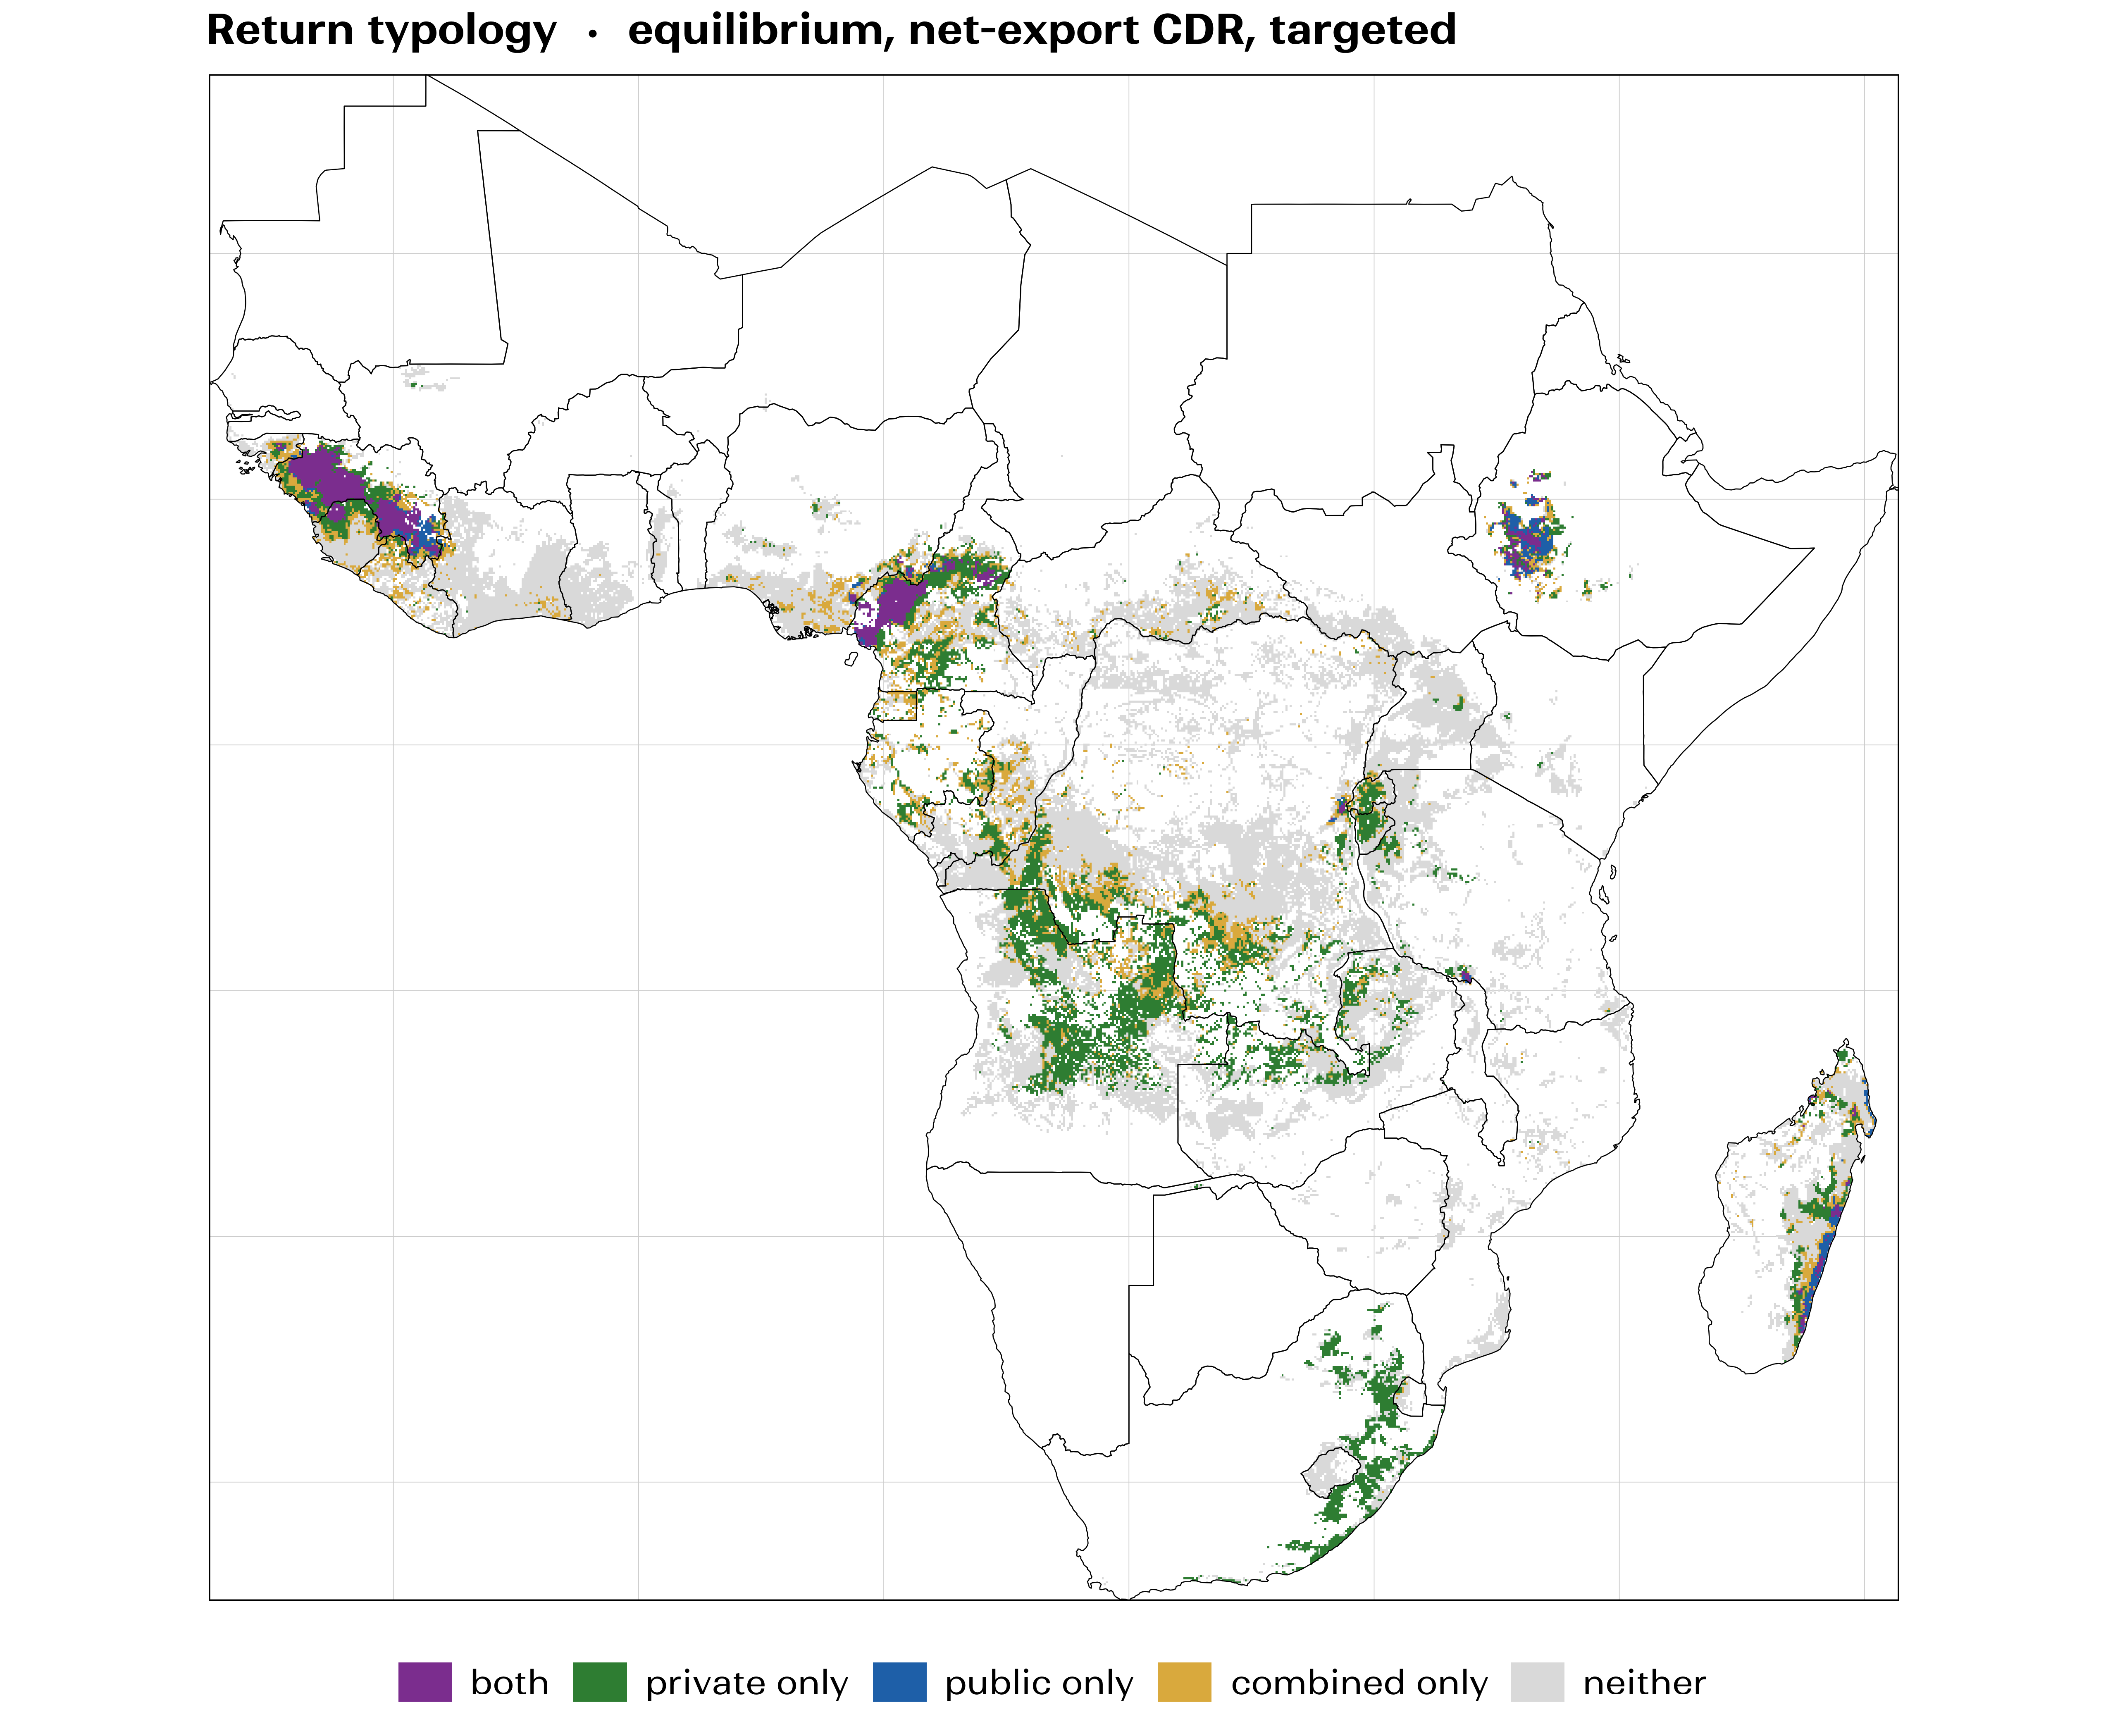
\includegraphics[width=\linewidth]{figures/fig-typology.png}
    \caption{Five-way return typology}
  \end{subfigure}\hfill
  \begin{subfigure}{0.42\linewidth}
    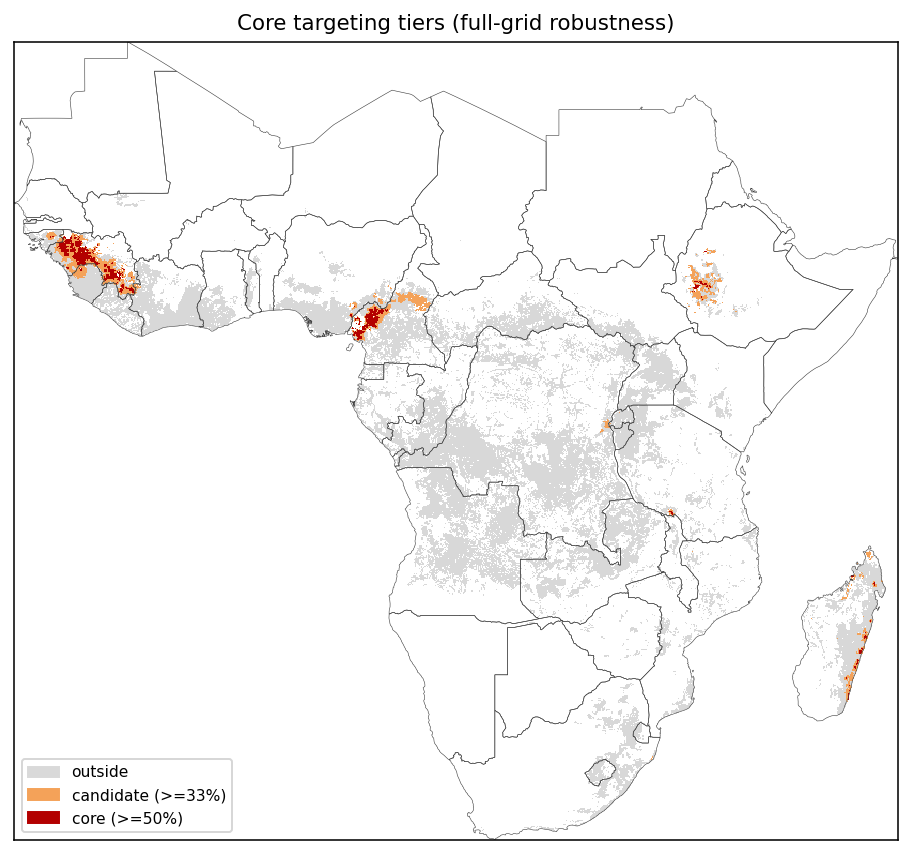
\includegraphics[width=\linewidth]{figures/fig-core.png}
    \caption{Core / candidate targeting tiers}
  \end{subfigure}
  \caption{Where each return carries the investment (left) and the robustness-based
  core targeting area (right). Maps use the conservative equilibrium, net-export
  accounting; the core concentrates in Cameroon, Guinea, the Ethiopian highlands,
  and coastal Madagascar.}
  \label{fig:envelopes}
\end{figure}

\subsection{The robust core}

No pixel stays in the intersection across more than 57\% of the 240-point
robustness grid --- the doubly-justified case is inherently parameter-sensitive.
On the robustness gradient (\autoref{tbl:core}), a plausible-central-band
cross-check independently gives $\sim$0.81\,Mha, so the two methods converge on
$\sim$0.7--0.8\,Mha of genuinely robust core land. It concentrates where acidic
soils, warm-wet climate, basalt proximity, and decent crop prices coincide:
Cameroon (0.42\,Mha core), Guinea (0.25), the Ethiopian highlands (0.05), and
Tanzania (0.02).

{\footnotesize
\begin{longtable}[]{@{}l>{\raggedright\arraybackslash}p{4.3cm}rrrr@{}}
\caption{Robustness-based targeting tiers (targeted allocation).}\label{tbl:core}\\
\toprule
Tier & Definition & Area (Mha) & Farms (M) & Value (\$M) & CDR (Mt) \\
\midrule
\endhead
Core & intersection under $\ge 50\%$ of grid & 0.74 & 0.45 & 663 & 13.1 \\
Candidate & intersection under $\ge 33\%$ of grid & 1.73 & 1.16 & 1,409 & 21.5 \\
\bottomrule
\end{longtable}
}

\subsection{What binds the public envelope}

The public envelope is small because durable removal is expensive per tonne, not
because the credit price is low. The area-weighted marginal-abatement cost
(\autoref{eq:mac}) across treated cropland is \textbf{p25 \$247, median \$305, p75
\$476/\tco} (\autoref{fig:mac}) --- set against a net credit price of only \$130
(\$150 less \$20 MRV). Only the cheapest $\sim$10--15\% of land clears, which is
why the public envelope is just 2.2\,Mha, and the price ladder is steeply convex
(\autoref{tbl:priceladder}).

\begin{figure}
  \centering
  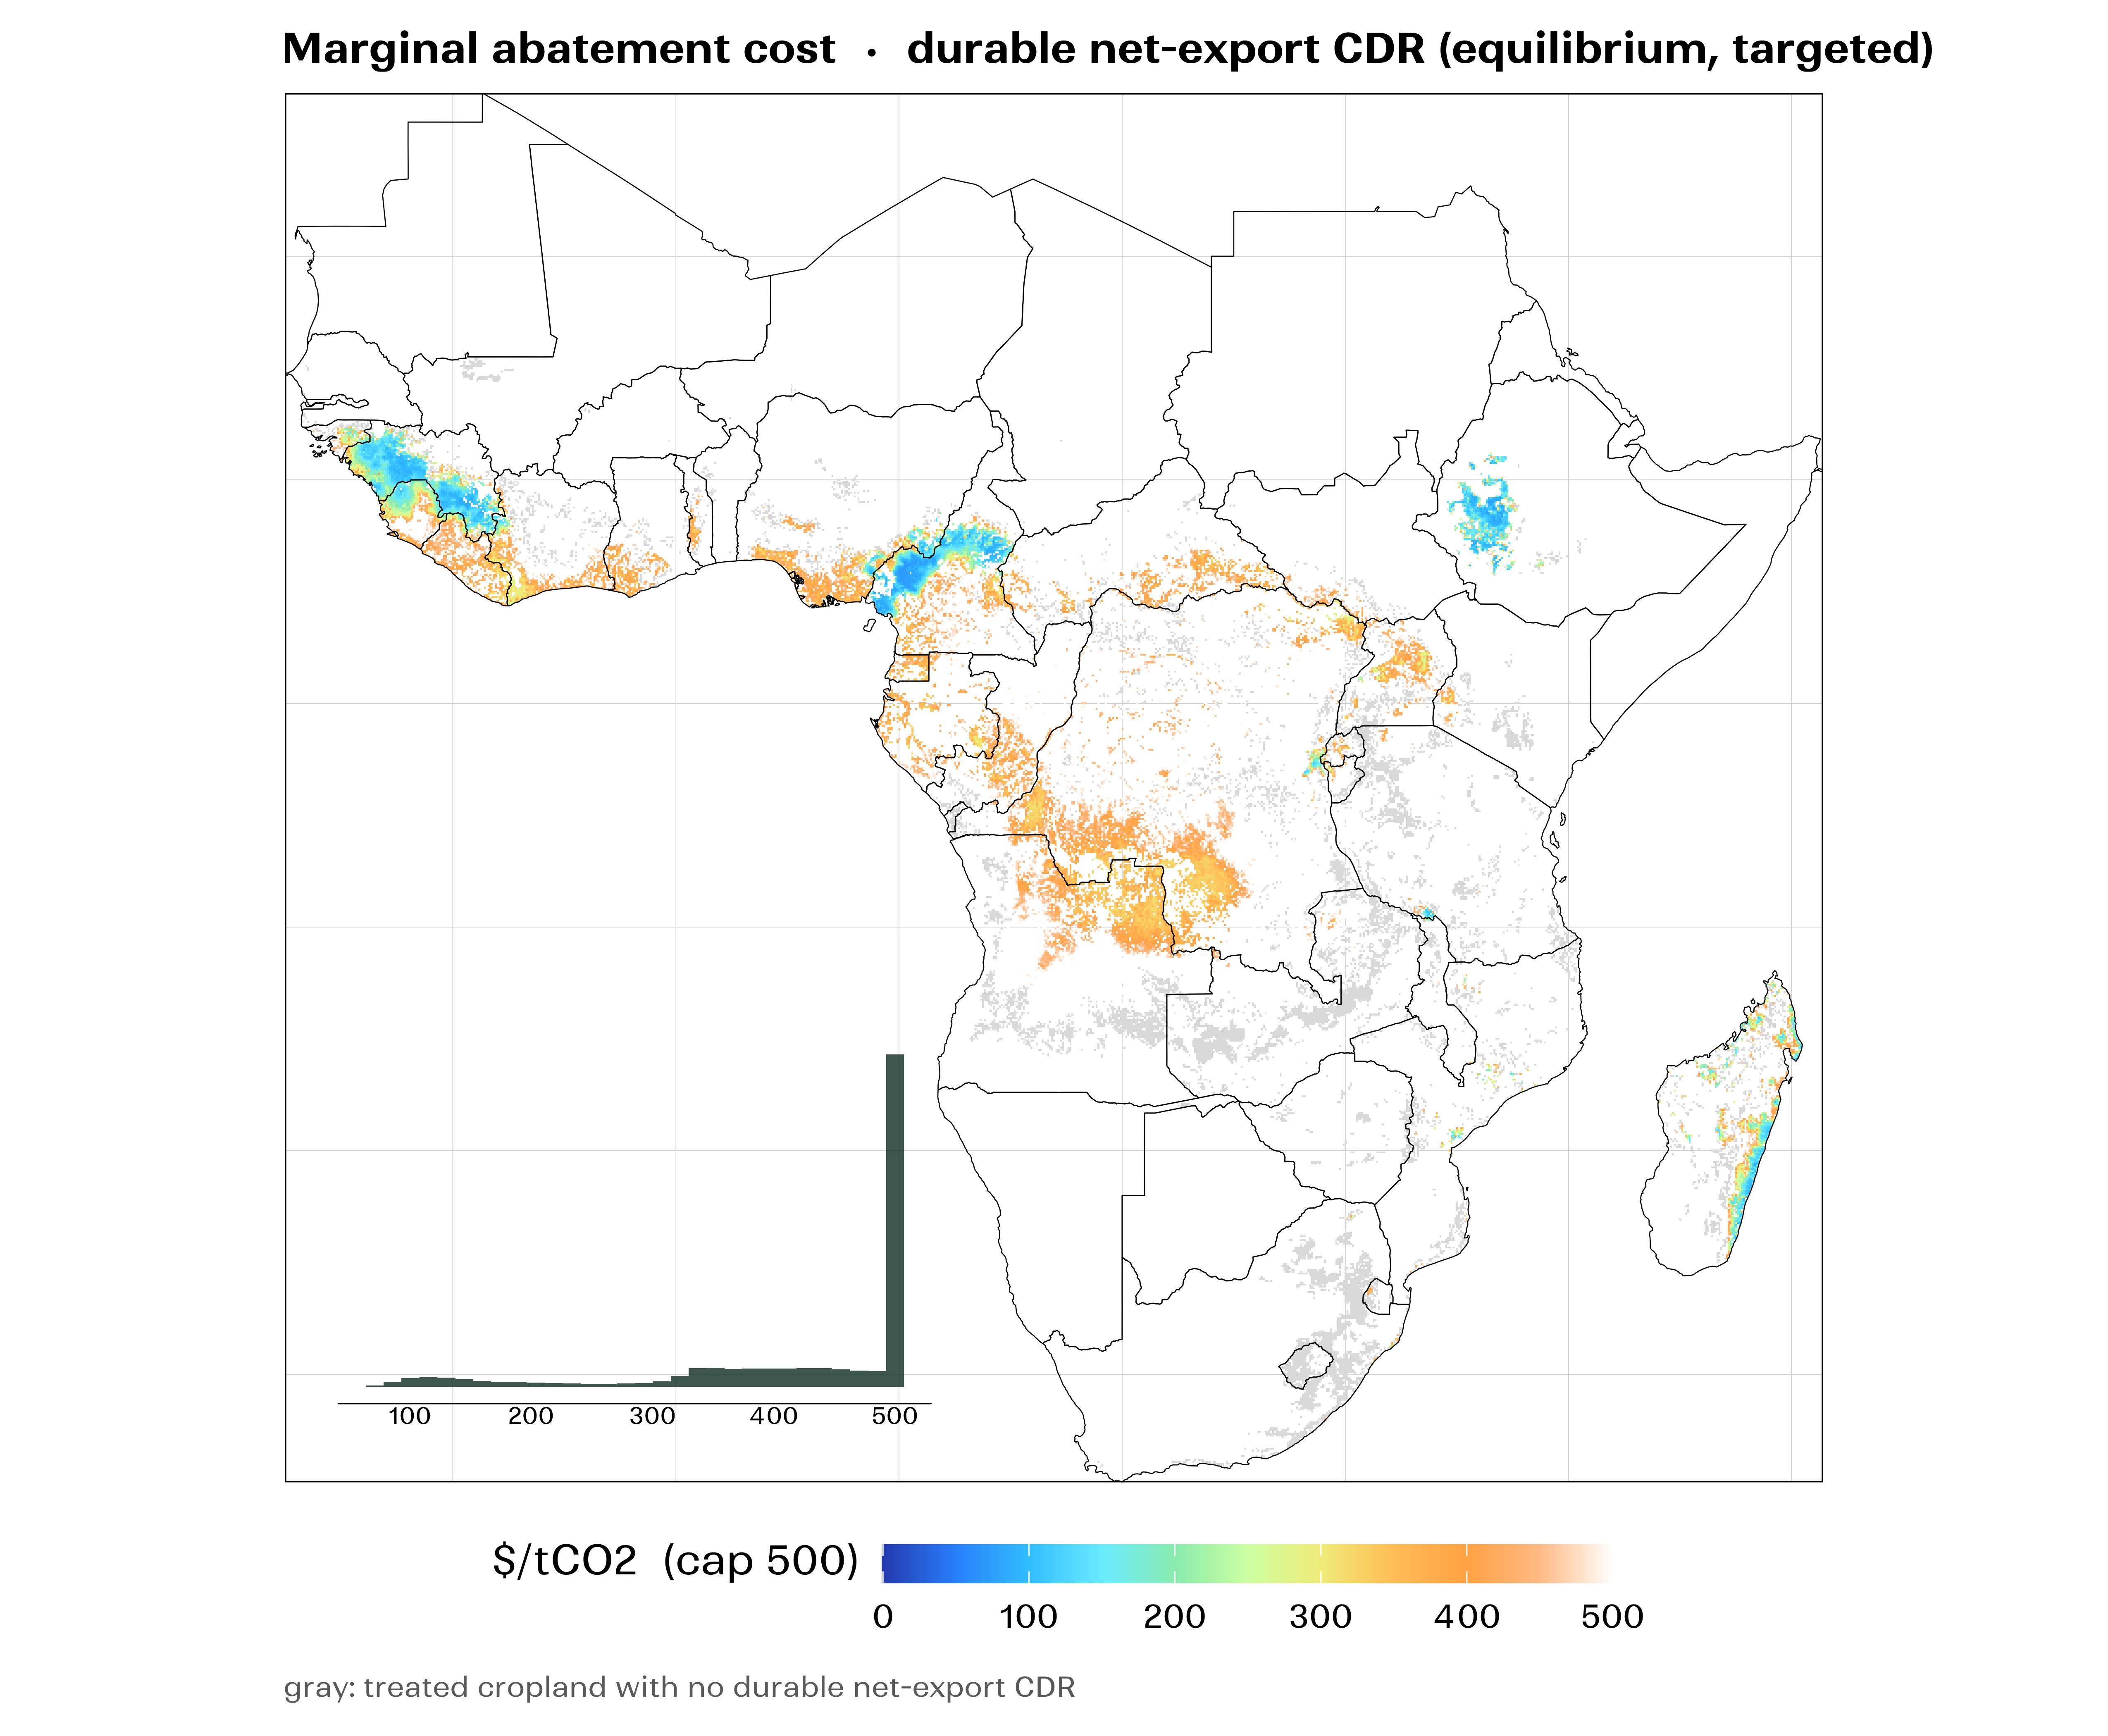
\includegraphics[width=0.82\linewidth]{figures/fig-mac.png}
  \caption{Marginal abatement cost of durable net-export CDR. The area-weighted
  distribution (inset histogram) sits well above the \$130/\tco\ net credit price,
  so only a small, cheap fraction of cropland is public-sufficient.}
  \label{fig:mac}
\end{figure}

\begin{longtable}[]{@{}rrr@{}}
\caption{Public-sufficient area and cumulative CDR as the VCM price
rises.}\label{tbl:priceladder}\\
\toprule
VCM price (\$/\tco) & Public area (Mha) & Cumulative CDR (Mt) \\
\midrule
\endhead
150 (current) & 2.23 & 25 \\
250 & 3.57 & 31 \\
300 & 7.52 & 51 \\
500 & 13.15 & 73 \\
1000 & 16.6 & 81 \\
\bottomrule
\end{longtable}

A lever comparison settles which knob matters: $+33\%$ carbon price widens the
public envelope by $+26\%$, $-33\%$ delivered cost by $+33\%$, $+33\%$ CDR rate by
$+23\%$ --- but \textbf{doubling the realised CDR rate widens it by $+181\%$}
(2.23 $\rightarrow$ 6.27\,Mha), beyond any plausible price or cost move. And a
one-at-a-time tornado on the intersection area confirms \textbf{delivered basalt
cost is the single dominant lever} (swing 5.62\,Mha over $\times0.5$--$2.0$),
larger than carbon price (2.80), CDR rate (2.38), and yield (0.89) --- so
targeting is first a logistics problem. Reassuringly, the yield benefit is the
\emph{least} sensitive input, which matters because it is also the most uncertain
(the Bayesian arm is prior-dominated).

\begin{keybox}
\textbf{Caveat on absolute area.} The committed \texttt{output-ssa-summary.csv}
figures reproduced in \autoref{tbl:ssa} (e.g.\ 137.9\,Mha ``profitable'') are
flagged \emph{stale} relative to the current \texttt{economics\_erw} rasters:
recomputing \texttt{erw-10}'s own definition on today's data gives
$\sim$9.9\,Mha combined-positive, consistent with the single-digit-Mha envelope
areas above. Read \autoref{tbl:ssa} for the \emph{relative} ranking of regimes and
allocations, and this section for the current-data footprint. Year-1 is also the
most optimistic regime; NPV and equilibrium shrink every envelope.
\end{keybox}

\section{What the results say}

\begin{enumerate}
\item \textbf{Targeted beats uniform.} Dosing to lime requirement dominates flat
application in every regime; uniform-50 destroys value.
\item \textbf{The CDR rate binds, not the carbon price} (\autoref{eq:mac}):
realised removal per tonne is small, so most cropland needs either a co-benefit
or a cheaper/finer feedstock to clear on carbon alone.
\item \textbf{Private and public returns are complementary}
(\autoref{fig:schematic}): the same acidity gradient that maximises yield relief
minimises exported carbon, and vice versa.
\item \textbf{The private case is larger than the public case}
(\autoref{sec:envelopes-results}): 8.2 vs.\ 2.2\,Mha targeted. Carbon finance is
decisive mainly on the 3.35\,Mha combined-only band, and \emph{least additional}
on the doubly-justified intersection --- with a robust core of only
$\sim$0.7--0.8\,Mha.
\item \textbf{Ranking and cap dominate the average}: a positive top decile exists
even where the mean is negative.
\end{enumerate}

% ==================================================================
\chapter{Assumptions, limitations, and roadmap}\label{ch:roadmap}

\section{Where the model uses defensible proxies (v1 flags)}

The CDR stream in particular is a first-order parameterisation. Each proxy below
is a deliberate, sourced simplification, not an oversight:
%
\begin{enumerate}
\item \textbf{Linear climate multipliers} (\autoref{eq:fmatmap}) stand in for
full reactive-transport kinetics; to be replaced by a Kanzaki-class form when
calibration data allow \citep{kanzaki2023}.
\item \textbf{Triangular pH factor} peaked at pH 5 (\autoref{eq:fph}) is a
defensible midpoint, not a calibrated curve.
\item \textbf{Reactive fraction $\phi_0 = 0.20$} is anchored to a single
temperate mesocosm \citep{lewis2021}.
\item \textbf{Grain-size exponent $\beta=0.5$} is the midpoint of an empirical
0.35--0.5 range, chosen to avoid a free parameter.
\item \textbf{Pedogenic loss} (\autoref{tbl:ped}) uses aridity bands, with MAP as
a fallback proxy for MAP/PET that over-deducts in cool highlands.
\item \textbf{EcoCrop as the operative yield response} captures tolerance ranges,
not basalt-specific uplift; the trial-anchored Bayesian arm is not yet run.
\end{enumerate}

\section{What the model does not represent}

N$_2$O and soil-compaction emissions from heavy application; Article 6 / credit
eligibility and corresponding adjustments; land tenure and who finances the
$\sim$\$600/ha upfront cost; industrial alkaline by-products (steel slag, cement
kiln dust) that could supply feedstock in basalt-poor regions; ultramafic
sources (excluded on safety grounds); a spatially varying MRV cost (a single flat
\$20/\tco\ is used); and any aggregator-level, as opposed to farmer-level,
economics.

\section{Roadmap: from v0 to v2}

\begin{keybox}
This report documents a \textbf{v0 screening model}: transparent, fast, and
honest about its proxies. It is meant to rank and compare, not to certify.
\end{keybox}

\begin{description}
\item[v0 (this report)] Interpretable multipliers; gross \emph{and} net bounds
carried side by side; every sensitive parameter swept. Good for ``where'' and
``how sensitive''.
\item[v1] Replace the reactive-fraction/climate block with an analytical
shrinking-core, particle-size-distribution dissolution model; run the Bayesian
yield arm on an expanded trial set.
\item[v2] Emulate a mechanistic 1-D reactive-transport model (SCEPTER-class) over
a designed experiment, and evaluate the fast surrogate per pixel --- the path to
credit-grade absolute numbers.
\end{description}

Because the v0 already carries gross and net bounds rather than a single point
estimate, and because its errors are largely monotone across the map, its
\emph{ranking} of locations is expected to be robust even as absolute tonnages
are refined --- which is exactly what a screening model needs to be right about.

% ==================================================================
\chapter{Reproducibility and provenance}\label{ch:repro}

\section{Run order}

\begin{verbatim}
erw-0   install packages
erw-1   soil layers + SSA/cropland grid
erw-2   SPAM crop layers
erw-3   feedstock chemistry + basalt rate
erw-4   crop EcoCrop parameter tables
erw-5   EcoCrop relative-yield rasters
erw-9   CDR surface (climate, pedogenic, net-export)
erw-basalt-access   logistics / delivered price
erw-energy-country  electricity + grid CI
[erw-yield-fit, erw-yield-predict]  optional Bayesian arm
erw-7   profitability (276 rasters)
erw-8   sensitivity sweeps
erw-supply   supply curves + deployment masks
erw-10, erw-11, erw-plot-maps   maps and tables
\end{verbatim}

\section{Environment and outputs}

R 4.5+ with \texttt{terra}, \texttt{geodata}, \texttt{sf}, \texttt{here},
\texttt{brms}, \texttt{malariaAtlas}, and the GAIA \texttt{limer} and
\texttt{Recocrop} packages. The profitability engine writes
\texttt{economics\_erw/\{allocation\}/\{crop\}\_\{regime\}.tif}, each carrying the
full decomposition (area, yield, loss, agronomic return, basalt rate and cost,
gross and net CDR, CDR revenue, and the combined / agro-only / CDR-only margins).
The constants catalogue with citations is \texttt{erw-parameters.md}; the CDR
derivation is \texttt{erw-cdr-calculations.pdf}.

% ---- References --------------------------------------------------
\backmatter
\renewcommand\bibname{{References}}
\bibliographystyle{apacite}
\addcontentsline{toc}{chapter}{References}
\nocite{*}
\bibliography{references}

\end{document}
